\section{Introduction}
Owing to the complicated and varied nature of phenomena in the \acrshort{thz} range, interpretation of the measured spectral properties requires calculation of the nature, frequency and intensity of the underlying modes. These, in turn, are calculated from the electronic ground state of the system. This is achieved by solving the many-body Schr\"{o}dinger equation (\acrshort{mbse}), which is shown in \Cref{eqn:MBSE}, and in this work this will be achieved using \acrfull{dft}~\cite{Kohn1965}.

\begin{equation}
\left( -\frac{1}{2}\sum_i\boldsymbol{\Delta}_i + \sum_i \boldsymbol{V}(\mathbf{r}_i) + \sum_{i\neq j}\frac{1}{ \lvert \mathbf{r}_i - \mathbf{r}_j \rvert } \right) \boldsymbol{\Psi} (\mathbf{r}_1, ..., \mathbf{r}_N) = \boldsymbol{E}\boldsymbol{\Psi} (\mathbf{r}_1, ..., \mathbf{r}_N)
\label{eqn:MBSE}
\end{equation}

\(\boldsymbol{\Delta}_i\) is the Laplace Operator acting on atom \(i\), \(\boldsymbol{V}(\mathbf{r}_i)\) is the potential energy, \(\mathbf{r}_i\) is the nuclear coordinates, \(\boldsymbol{\Psi}\) is the wavefunction and \(\boldsymbol{E}\) is the energy of the system. Initially, \acrshort{dft} was only used for very simple and uniform systems such as metals but development over the last few decades has enabled its use in far more complicated systems and studying chemical phenomena, such as pharmaceutically relevant compounds~\cite{Berzins2020}, phase transformations in crystal structures~\cite{Ruggiero2018, Paul2019}, nanomaterial properties~\cite{Makkar2021} and amino acids~\cite{Hachtel2019}. Other methods have been developed for attempting this and are widely used in the context of an isolated molecule in the gas phase. Whilst they can be used for periodic systems, they either tend to not match experimental data or become extremely expensive computations that can be unfeasible for large systems.

This chapter will describe \acrshort{dft} and the methodology of applying it to useful chemical systems, followed by a description of the software packages, general procedure and calculation parameters used. 

\section{Density Functional Theory}
\label{sec:DFTheory}
\subsection{Solving the Many Body Schr\"{o}dinger Equation}
Underpinning most quantum mechanical theories, \acrshort{dft} also uses the Born\nobreakdash-Oppenheimer approximation which states that any motion of a nucleus is much slower than the motion of an electron. This allows for an instantaneous response by the electron to the nucleus and as such, nuclei are treated as fixed in space, reducing the number of contributions to the total energy of the system. Attempting to solve the \acrshort{mbse} is too complex for all but the smallest systems so a number of simplifications have been developed over the years. In particular, the electron orbitals are defined to be one-electron non-interacting orbitals where:

\begin{equation}
\boldsymbol{\Psi} (\mathbf{r}_1, ..., \mathbf{r}_N) \xrightarrow{} \{\psi_1(\mathbf{r}),  \psi_2(\mathbf{r}), ..., \psi_N(\mathbf{r})\}
\end{equation}

\begin{equation}
\boldsymbol{\Psi}(\mathbf{r}_1, ..., \mathbf{r}_N) = \prod_i^N \psi_i (\mathbf{r}_i)
\end{equation}

These assumptions allow the separation of the total energy of the system, \(\boldsymbol{E}_{tot}\), into the following terms:

\begin{equation}
\boldsymbol{E}_{tot} = \boldsymbol{E}_{KE} + \boldsymbol{E}_{H} + \boldsymbol{E}_{Z} + \boldsymbol{U}_{Z} + \boldsymbol{E}_{XC} 
\label{eqn:GSComponents}
\end{equation}

where \(\boldsymbol{E}_{KE}\) is the kinetic energy of the electrons, \(\boldsymbol{E}_{H}\) is the Hartee energy which is the Coulombic potential energy, \(\boldsymbol{E}_{Z}\) is the potential energy between the electrons and the nuclei, \(\boldsymbol{U}_{Z}\) is the potential energy between the nuclei and \(\boldsymbol{E}_{XC}\) is the correlation exchange energy between the electrons. As these electron orbitals are non-interacting, each one has its own associated coordinate system in three dimensions. This results in a calculation that increases in magnitude as more electrons were added, which meant that calculations involving large amounts of electrons slowed down dramatically. Kohn, Honenburg and Sham~\cite{Kohn1965, Hohenberg1964} developed a method that attempted to solve this. By defining each term in \Cref{eqn:GSComponents} as a functional dependent on the electron density, \(\rho\), the number of coordinates that needed to be calculated was reduced from \(3N\) to three. The total energy of the system can now be represented as:

\begin{equation}
\boldsymbol{E}[\rho] = \boldsymbol{E}_{KE}[\{\psi_i[\rho]\}] + \boldsymbol{E}_{H}[\rho] + \boldsymbol{E}_{Z}[\rho] + \boldsymbol{U}_{Z}[\rho] + \boldsymbol{E}_{XC}[\rho]
\end{equation}

The electron density is calculated using one electron orbitals, represented using basis sets, which are shown by:

\begin{equation}
\boldsymbol{\rho}(\mathbf{r}) = \sum_{i}^{\boldsymbol{N}} \lvert {\psi_i(\mathbf{r})} \rvert ^2
\end{equation}

This allows orbitals to be calculated as a linear combination of atomic orbitals and this is discussed further in \Cref{subsec:bloch} and \Cref{subsec:pseudopot}. The Kohn\nobreakdash-Sham equation, which is a modified \acrshort{mbse}, is used to calculate these one electron orbitals with:

\begin{equation}
\left( -\frac{1}{2}\boldsymbol{\Delta} + V_z(\mathbf{r}) + V_H[\rho](\mathbf{r}) + V_{XC}[\rho](\mathbf{r)}\right) \psi_i(\mathbf{r}) =  \epsilon_i \psi_i (\mathbf{r})
\end{equation}

Each term can be calculated exactly with the exception of the final term, \(V_{XC}[\rho]\). This is the exchange correlation energy and represents the interaction between the electrons. These are described as functionals and there are many possible approximations for this, the simplest being the \acrfull{lda}~\cite{Sahni1988}. This is where the electron density is assumed to be homogeneous. More complex functionals incorporate the gradient of the electron density as well and the simplest of these is called the \acrfull{gga}~\cite{Perdew1996}. These can often be broken into separate exchange and correlation components that can be mixed to form new functionals such as meta\nobreakdash-\acrshort{gga}s~\cite{Furness2021} and hybrid functionals such as B3LYP~\cite{Stephens1994}. B3LYP is often used by the chemical community for small molecules but is computationally expensive. In this work, a version of \acrshort{gga} developed by Perdew \textit{et. al.}~\cite{Perdew1996_2} has been used throughout this work and is referred to as the \acrfull{pbe} functional. This is a relatively simple functional that this group has previously shown can provide accurate results and is computationally efficient when compared to hybrid and meta functionals.

\subsection{Periodic Systems}
\label{subsec:bloch}
Whilst simplifying the \acrshort{mbse} drastically decreases the magnitude of the calculation, for crystals and other extended systems further simplification is needed as the number of electrons is still on the order of approximately \(10^{23}\). This is done by considering that the unit cell, the smallest infinitely repeating section of the crystal, must have the same orbitals at the same position in the unit cell regardless of where that is in the crystal. This is described by:

\begin{equation}
\psi_{n\mathbf{k}}(\mathbf{r} + \mathbf{R}) = \psi_{n\mathbf{k}}(\mathbf{r})e^{i\mathbf{k}\mathbf{R}}
\end{equation}

\begin{equation}
\psi_{n\mathbf{k}}(\mathbf{r}) = u_{n\mathbf{k}}(\mathbf{r})e^{i\mathbf{k}\mathbf{R}}
\end{equation}

\begin{equation}
u_{n\mathbf{k}}(\mathbf{r} + \mathbf{R}) = u_{n\mathbf{k}}(\mathbf{r})
\end{equation}

where \(\mathbf{R}\) is any lattice vector, \(n\) is the band index and \(\mathbf{k}\) is the Bloch vector, where orbitals are calculated at each Bloch vector. These Bloch vectors are described in the reciprocal lattice, \(u\), which represents the Fourier Transform of the physical lattice. The first \acrfull{bz} represents the primitive cell in this reciprocal space and these Bloch vectors are constrained to this area. The centre of the \acrshort{bz} is called the `Gamma' point, typically \(\Gamma\)-Point, and only phonons involved with this centre are \acrshort{ir}\nobreakdash-active. The most desired parameters are extracted by integrating over the \acrshort{bz}:

\begin{equation}
\rho(\mathbf{r}) = \frac{1}{\Omega_{BZ}} \sum_n \int_{BZ} f_{n\mathbf{k}} \lvert \psi_{n\mathbf{k}}(\mathbf{r}) \rvert^2 d\mathbf{k}
\end{equation}

where \(\Omega_{BZ}\) is a constant dependent on the lattice and \(f_{n\mathbf{k}}\) are the Fourier component of the integration. This is costly and unnecessary as orbitals that are close together are typically identical or very similar. This means the integral can be replaced by a weighted sum over a grid of points and these points are called k\nobreakdash-points. In this work, each calculation used the Monkhorst-Pack~\cite{Monkhorst1976} method for the description of k-points. The number of points required can be further reduced through symmetry operations and this reduced calculated area is called the irreducible \acrshort{bz}. The equation becomes: 

\begin{equation}
\rho(\mathbf{r}) = \sum_{n\mathbf{k}} \omega_\mathbf{k} f_{n\mathbf{k}} \lvert \psi_{n\mathbf{k}}(\mathbf{r}) \rvert^2 d\mathbf{k}
\end{equation}

where \(\omega_\mathbf{k}\) is a weighting factor. The number of these points can be reduced for calculation speed and increased for computational accuracy and the details of how these were chosen for the calculations in this thesis will be discussed in \Cref{subsubsec:convergence}. 

\begin{figure}
    \centering
    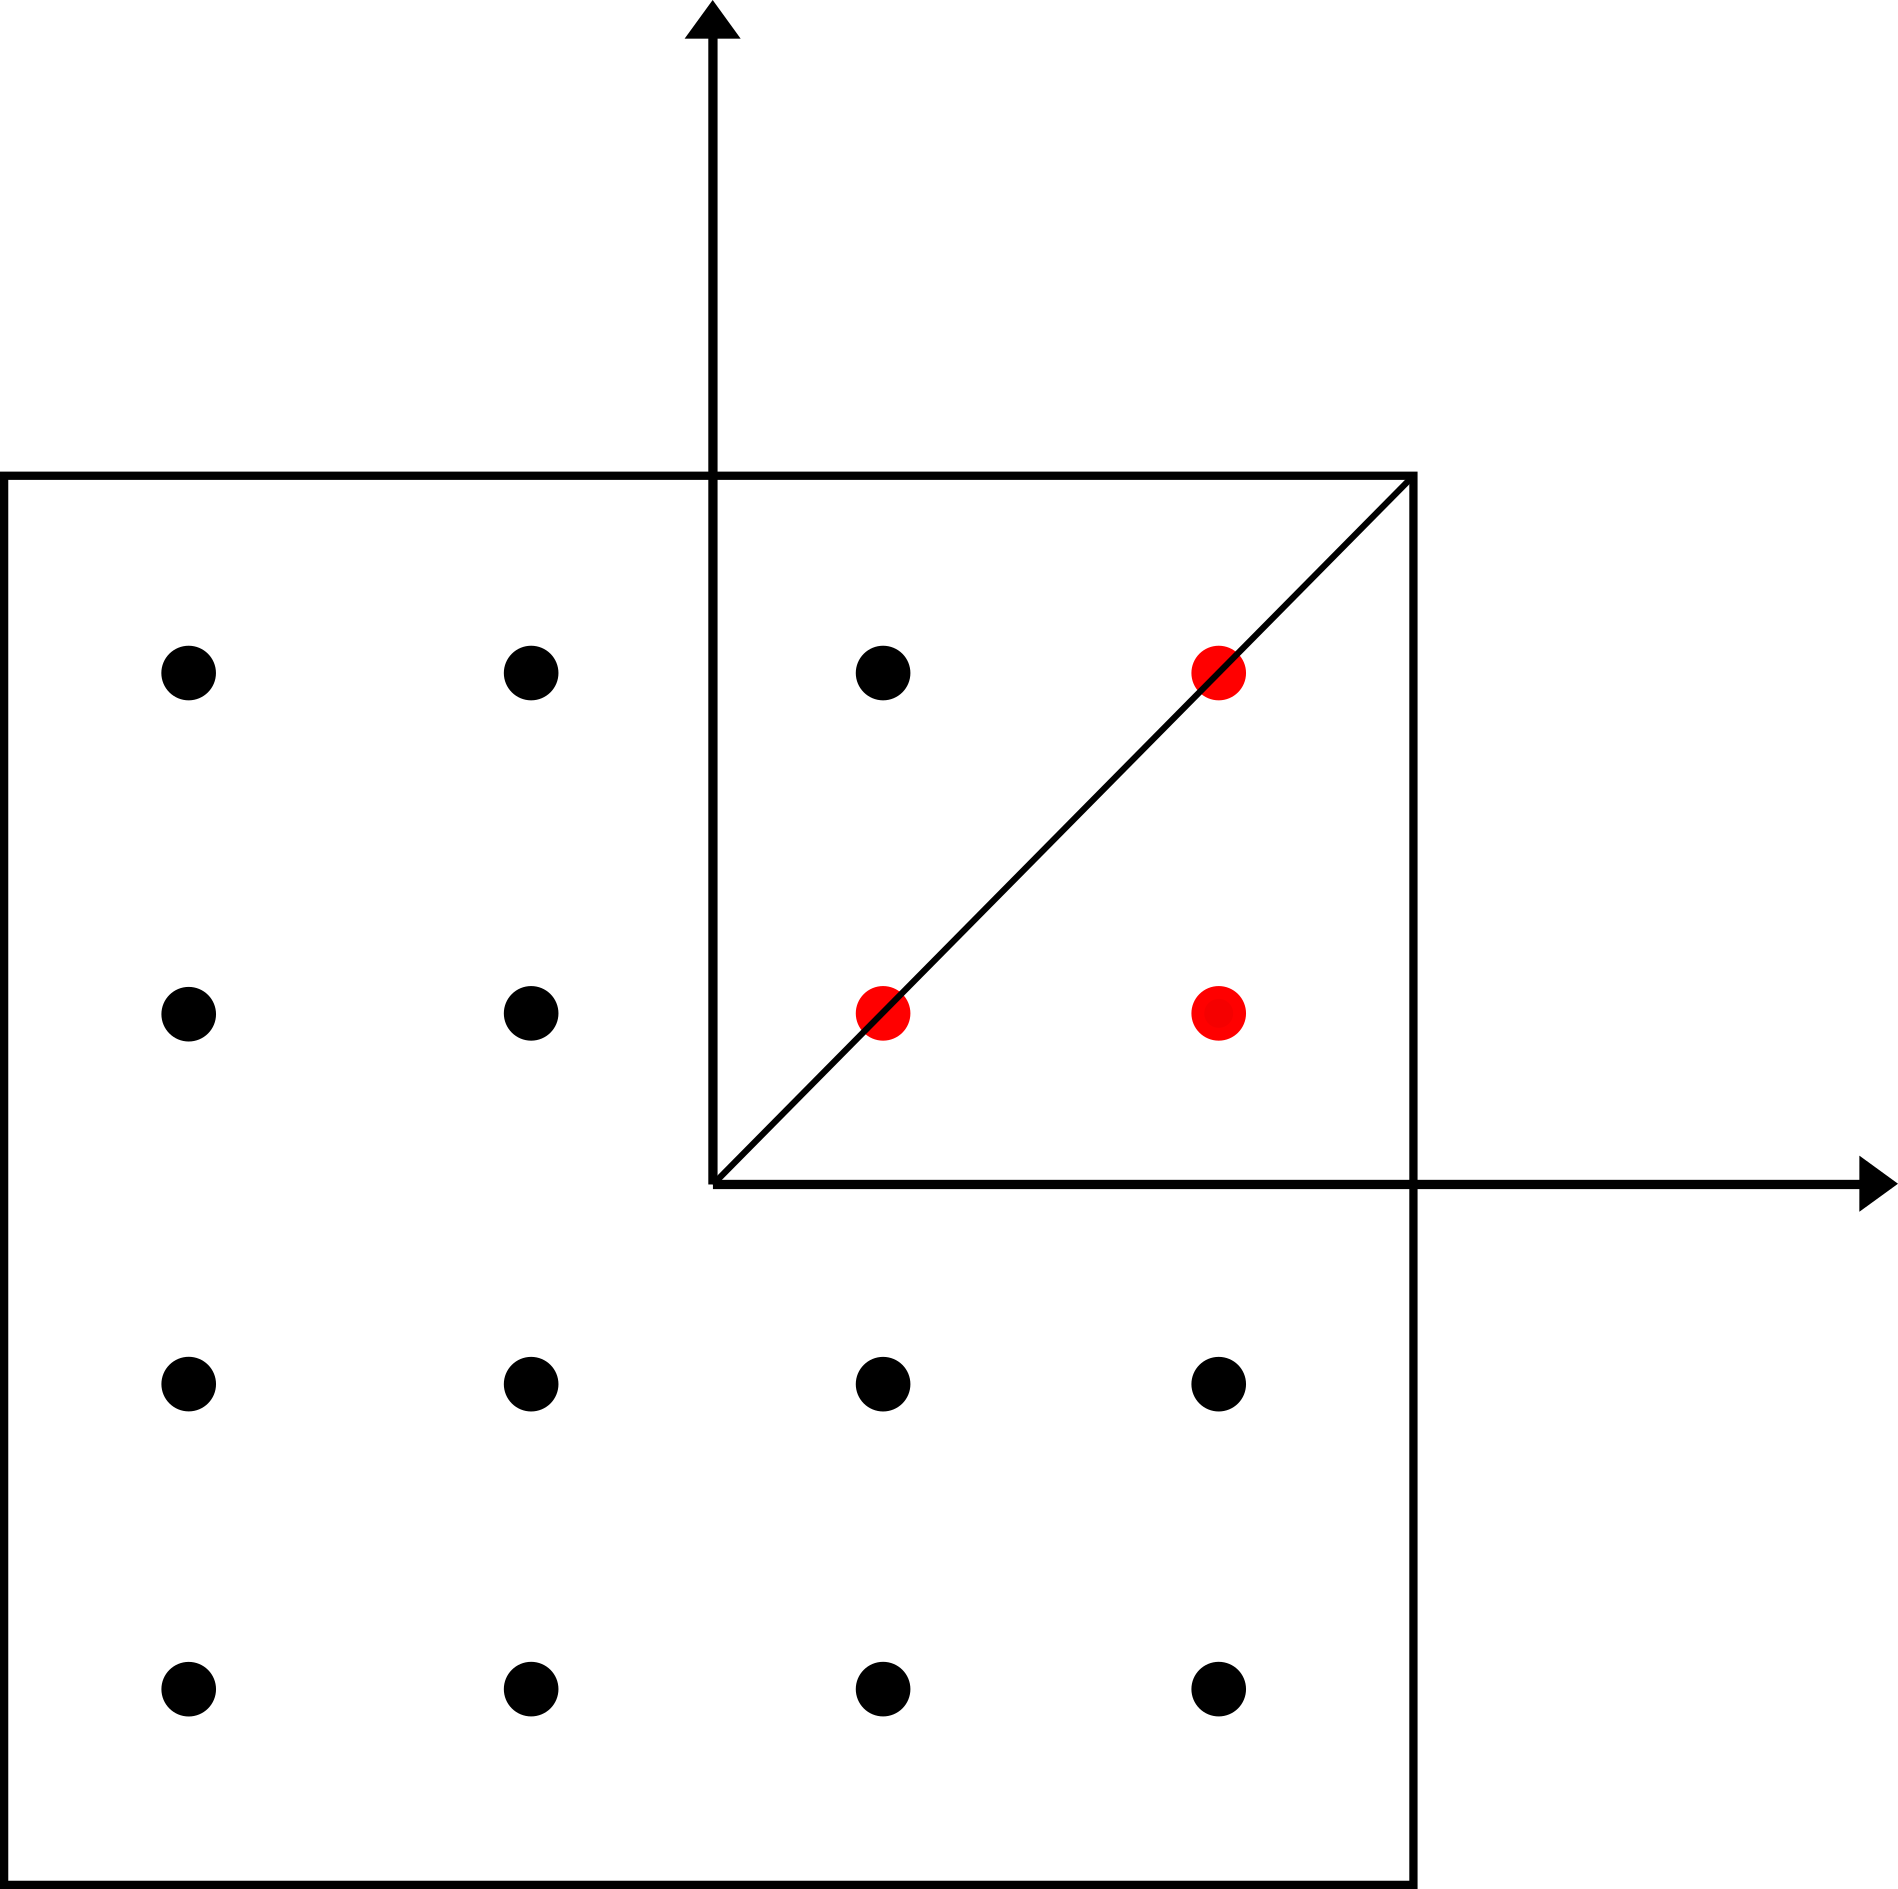
\includegraphics{Figures/Misc/Theory/BZ+IBZ.png}
    \captionsetup{font = footnotesize, justification = centering}
    \caption[A Schematic of the Brillouin Zone]{A schematic of the \acrshort{bz}. The black dots represent all required k-points and the red dots represent the k-points that can be mapped onto all others using symmetry operations. This is called the irreducible Brillouin Zone.}
    \label{fig:BZIBZ}
\end{figure}

For single molecule calculations performed by those in the chemical community, the molecular orbitals themselves are typically represented by basis sets that are constructed from localised functions centred around each atomic nucleus~\cite{Huzinaga1985}. These can be Slater Type Orbitals (\acrshort{sto}), which have the form \(\boldsymbol{r^ne^{-\zeta r}}\) or Gaussian Type Orbitals (\acrshort{gto}), which have the form \(\boldsymbol{e^{-r}}\). \acrshort{sto}s typically are better at representing the shape of the wavefunction but are more complex to integrate over whilst \acrshort{gto}s are worse at representing the wavefunction but the integral can be more easily calculated. These are generally combined to give hybrid orbitals the smallest of which is \acrshort{sto}\nobreakdash-3G~\cite{Halgren1978}, which combine the advantages of both. Whilst these can be used in solid\nobreakdash-state, these can be difficult to implement owing to translational symmetry in the solid. Despite this, these are used by CP2K~\cite{Khne2020} and Crystal17~\cite{dovesi2020crystal} but a majority of \acrshort{dft} codes use plane waves. One method of circumventing this has been to use plane waves instead~\cite{Hohenberg1964}. This gives the wavefunction the form: 

\begin{equation}
\psi_{n\mathbf{k}}(\mathbf{r}) = \frac{1}{\Omega^{0.5}} \sum_{\boldsymbol{G}} C_{\boldsymbol{G}n\mathbf{k}}e^{i(\boldsymbol{G}+\mathbf{k})\mathbf{r}}
\end{equation}

The reduced cost arises from the easy conversion between reciprocal and real space and the ease of calculating certain parameters in each space, such as the exchange correlation and Hartree potentials:

\begin{equation}
C_{\mathbf{r}n\mathbf{k}} = \sum_G C_{\boldsymbol{G}n\mathbf{k}} e^{i\boldsymbol{G}\mathbf{r}} \overset{FFT}{\leftrightarrow} C_{\mathbf{G}n\mathbf{k}} = \frac{1}{N_{FFT}} \sum_{\mathbf{r}} C_{\boldsymbol{r}n\mathbf{k}} e^{-i\boldsymbol{G}\mathbf{r}}
\end{equation}

As with localised basis sets, an infinite number of either is required to exactly represent the wavefunction which is not practical. Whilst the localised basis sets are constructed from a pre\nobreakdash-determined number of orbitals, plane waves are constrained by defining a cut\nobreakdash-off energy that provides a limit to the maximum energy of any constituent plane wave. Reducing this cut\nobreakdash-off energy reduces the accuracy of the calculation but also reduces its cost and the reverse is also true. This parameter is selected on a per\nobreakdash-calculation basis and this is discussed further in \Cref{subsubsec:convergence}. The key advantage is that one number can be used to smoothly increase the accuracy of the calculation whereas this is not possible with localised basis sets.

\subsection{Pseudopotentials}
\label{subsec:pseudopot}
When considering systems that contain elements heavier than He, the electrons that are typically involved in covalent bonding are in outer orbitals called valence orbitals. The remaining electrons are referred to as core electrons and do not take part in any bonding processes. Whilst \acrshort{dft} does not model the electrons themselves, but the electron density, calculating this to a high degree of accuracy for the area in space where these core orbitals will be will not significantly improve the accuracy of the calculation but may significantly increase its computational cost as a much finer mesh of k\nobreakdash-points will have to be used. As such, the concept of a pseudopotential was developed to model the core electrons collectively.

Traditional pseudopotentials typically take two forms; `norm\nobreakdash-conserving' and `ultrasoft'. Norm\nobreakdash-conserving pseudopotentials~\cite{Hamann1979} must satisfy two conditions. Firstly, inside a specified cut\nobreakdash-off radius, the normalisation of a pseudo\nobreakdash-wavefunction should be equal to the normalisation of the all\nobreakdash-electron wavefunction. The other condition is that the wavefunctions should be equal outside of this cut\nobreakdash-off radius. Ultrasoft pseudopotentials~\cite{Vanderbilt1990} relax this constraint by not requiring that the normalisations of the wavefunctions to be exactly equal. This reduces their computational cost further but at the expense of their ability to be implemented in different chemical environments without testing their suitability. Whilst these were originally developed for localised basis sets, they are also used when modelling the wavefunction using plane waves.

Another approach to this problem is the \acrfull{paw} method~\cite{Blochl1994}. This works through construction of a transformation operator that can calculate the properties of the all\nobreakdash-electron system from the pseudo\nobreakdash-wavefunction. These are typically pre\nobreakdash-calculated for a given atomic environment and therefore further save computational expense. \acrshort{paw} potentials combine the computationally efficient advantages of pseudopotentials but provide the ability to still calculate the all\nobreakdash-electron material properties if required. This can facilitate a lower plane wave cut\nobreakdash-off energy than available if you needed to use norm\nobreakdash-conserving pseudopotentials. These will be used for all calculations in this work as these are available with VASP~\cite{Hafner2008} and this is the code used in this work.

\subsection{Calculation of Vibrational Modes}
\label{subsec:vibmodestheory}
The frequencies and intensities of any phonon modes that are present in the system can be calculated by determining the effect of ion displacement on the energy of the system. This can be calculated by expanding the energy as a Taylor series with the form:

\begin{equation}
\boldsymbol{E} = \boldsymbol{E}_0 + \frac{\delta \boldsymbol{E}}{\delta u}.u + \frac{1}{2!} \frac{\delta^2 \boldsymbol{E}}{\delta u^2}.u^2 + \frac{1}{3!} \frac{\delta^3 \boldsymbol{E}}{\delta u^3}.u^3 + ...
\label{eqn:ETaylor}
\end{equation}

where \(\boldsymbol{E}\) is the total energy of the system, \(\boldsymbol{E}_0\) is the energy of the system at equilibrium  and \(\boldsymbol{u}\) is the displacement from equilibrium position. When an ion is displaced, each other ion that experiences a force will oscillate around a new equilibrium position. Whilst \acrshort{dft} can be used to calculated any term in \Cref{eqn:ETaylor}, this becomes more computationally expensive for each included term. By assuming the oscillation is harmonic, the harmonic vibrational frequencies can be extracted. The key assumption underpinning this is that at its equilibrium position, movements of an ion will result in a harmonic potential energy distribution. This assumption is called the harmonic approximation. Third order terms and higher are set to be zero in this approximation and do not have to be calculated, but contain information about any anharmonicity in the system. These can be important in a wide range of systems and conditions and this will be discussed further in \Cref{ch:qha}. 

At this new equilibrium position, the gradient of the potential energy is zero and so the first term in \Cref{eqn:ETaylor} becomes zero. The energy now is defined as:

\begin{equation}
\boldsymbol{E} = \boldsymbol{E}_0 + \frac{1}{2} \sum \boldsymbol{u}_{\alpha, \kappa}.\Phi_{\alpha, \alpha'}^{\kappa, \kappa'}.\boldsymbol{u}_{\kappa', \alpha'}
\end{equation}
where:
\begin{equation}
\Phi_{\alpha, \alpha'}^{\kappa, \kappa'} =  \frac{\delta^2 \boldsymbol{E}}{\delta \boldsymbol{u}_{\alpha, \kappa} \delta \boldsymbol{u}_{\alpha', \kappa'}}
\end{equation}

where \(\alpha\) is the Cartesian direction in which the displacement occurs, \(\kappa\) is the label of each atom in the considered unit cell and \(\Phi_{\alpha, \alpha'}^{\kappa, \kappa'}\) is the force constant matrix of the system, which effectively represents the effect on the force experienced on an atom by moving another. One solution to this differential equation is modelling the displacement with a travelling wave:

\begin{equation}
\boldsymbol{u}_{\alpha, \kappa} = \epsilon_{m, \alpha, \kappa, \boldsymbol{q}}e^{i\boldsymbol{q}.\boldsymbol{R}_{\alpha, \kappa} - \omega t}
\end{equation}

By differentiating the energy equation to get the force and substituting in the trial solution, the vibrational mode frequencies at the \(\Gamma\)\nobreakdash-point can be calculated from:

\begin{equation}
\boldsymbol{D}_{\alpha, \alpha'}^{\kappa, \kappa'} (\boldsymbol{q}) \epsilon_{m, \alpha, \kappa, \boldsymbol{q}} = \omega^2_{m,\boldsymbol{q}} \epsilon_{m, \alpha, \kappa, \boldsymbol{q}}
\end{equation}

where:
\begin{equation}
\boldsymbol{D}_{\alpha, \alpha'}^{\kappa, \kappa'} (\boldsymbol{q}) = \frac{1}{\sqrt{m_{\kappa} m_{\kappa'}}} \sum \boldsymbol{\Phi}_{\alpha, \alpha'}^{\kappa, \kappa'} e^{-i\boldsymbol{q}.\boldsymbol{R}}
\end{equation}

\(\boldsymbol{D}_{\alpha, \alpha'}^{\kappa, \kappa'} (\boldsymbol{q})\) is referred to as the dynamical matrix and is the Fourier Transform of the force constant matrix, \(\Phi_{\alpha, \alpha'}^{\kappa, \kappa'}\). The eigenvalues of this equation are the vibrational mode frequencies and are calculated by taking the square root of \(\omega^2_{m,\boldsymbol{q}}\) and the eigenvector \(\epsilon_{m, \alpha, \kappa}\) is the atomic displacements of this mode. \(m\) refers to the mass of the atom and \(\boldsymbol{q}\) is the wavevector.

There are two main methods for calculating \(\boldsymbol{D}_{\alpha, \alpha'}^{\kappa, \kappa'} (\boldsymbol{q})\); numerically, using the finite displacement method and analytically, using \acrfull{dfpt}~\cite{Giannozzi2005}. Finite displacement~\cite{Kresse1995, Parlinski1997} works through displacing an ion by a small distance, \(\pm u\), and calculating the resulting forces on every other ion in the system for each direction of the displacement. Using the central-difference formula, the force matrix can be calculated:

\begin{equation}
\frac{\delta F_{\kappa, \alpha}}{\delta u} \approx \frac{F_{\kappa, \alpha}^+ - F_{\kappa, \alpha}^-}{2u} = \frac{\delta^2 E}{\delta u_{\kappa, \alpha} \delta u_{\kappa', \alpha'}}
\end{equation}

This completes a row of \(\boldsymbol{D}_{\alpha, \alpha'}^{\kappa, \kappa'} (\boldsymbol{q})\) and by displacing along the other two Cartesian coordinates, the rows associated with this atom are completed. Through repetition over each atom in the unit cell, which can be reduced through symmetry operations, the full dynamical matrix can be calculated. 

\acrshort{dfpt} determines this response through use of perturbation theory~\cite{Baroni2001}, which allows calculation of the dynamical matrix from an analytical expression relating the energy of the electron density to a perturbation of ionic position. This technique is not used in this work to calculate the dynamical matrix owing to the 48 hour limit on calculations run on ARC3, the University of Leeds High Performance Computing facility. As VASP~\cite{Hafner2008}, the main \acrshort{dft} software package used in this work, is currently is not able to restart this calculation after it is stopped and this work has focused on \acrshort{alm}, which required more than 48 hours to complete, \acrshort{dfpt} has not been used in this work to calculate phonon frequencies. 

However, it is used to calculate the Born effective charges~\cite{Gonze1997}. These are the coefficients that relate a polarisation along the unit cell in a particular direction to the corresponding displacement this causes. As, for \acrshort{tds}, many samples are diluted using a non\nobreakdash-absorbing medium, the production of an experimentally\nobreakdash-comparable simulated spectrum from the frequencies and intensities of the calculated modes can be challenging. This and how intensities are extracted from the Born effective charges will be discussed in \Cref{subsec:pdielec}.

\subsection{Dispersion Corrections}
\label{subsec:dcs}
Whilst \acrshort{dft} is effective at modelling intramolecular forces, it is comparatively much weaker with intermolecular forces such as London dispersion forces~\cite{Kristyan2004}. This poses a problem when investigating large complex molecules as often these forces can play a significant role in these systems and the thermodynamic properties can significantly depend on them. As such, numerous empirical dispersion corrections have been created to attempt to recreate these interactions within \acrshort{dft} with minimal computational cost. Owing to the significant sensitivity of calculated spectral features to small fluctuations of electron density, including interactions such as London dispersion forces into the calculation is of vital importance. Most functionals, such as the \acrshort{pbe} functional used in this work, do not tend to appropriately describe higher order electron correlational effects such as these. One method of achieving this is to add a correction term to the energy for each calculation step, often called a dispersion correction (\acrshort{dc}). Whilst there are alternative methods for incorporating noncovalent interactions in \acrshort{dft}~\cite{Kozuch2010}, using \acrshort{dc}s such as those examined in this work are comparatively much less costly and these are now an easily implemented part of most quantum calculation packages.
In total, five \acrshort{dc}s were evaluated in \Cref{ch:ivdw} and will be described here. The oldest and simplest was the \acrshort{dft}-D2~\cite{Grimme2006} \acrshort{dc} which corrects the energy of the system using the formula:

\begin{equation}
\boldsymbol{E}_{D2} = -\frac{1}{2}\ \sum_{i=1}^{\boldsymbol{N}_{at}} \sum_{j=1}^{\boldsymbol{N}_{at}} \sideset{}{'}\sum_{\boldsymbol{L}} \frac{\boldsymbol{C}_{6ij}}{\boldsymbol{r}_{ij,\boldsymbol{L}}^6} \boldsymbol{f}_{d,6}(\boldsymbol{r}_{ij, \boldsymbol{L}}) 
\end{equation}

where \( f(r_{ij}) \) is the damping factor and is given by:

\begin{equation}
\boldsymbol{f}_{d,6}(\boldsymbol{r}_{ij}) = \frac{\boldsymbol{s}_6}{1 + \boldsymbol{e}^{-d(\boldsymbol{r}_{ij} / (\boldsymbol{s}_{\boldsymbol{R}} \boldsymbol{R}_{0ij})-1)}} 
\end{equation}

Parameters \( \boldsymbol{C}_{6ij} \) and \( \boldsymbol{R}_{0ij} \) are computed using:

\begin{equation}
\boldsymbol{C}_{6ij} = \sqrt{\boldsymbol{C}_{6ii} \boldsymbol{C}_{6jj}} 
\end{equation}

\begin{equation}
\boldsymbol{R}_{0ij} = \boldsymbol{R}_{0i} + \boldsymbol{R}_{0j} 
\end{equation}

\(\boldsymbol{N}_{at}\) is the number of atoms and \(\boldsymbol{L}\) is all translations of the unit cell. When \(\boldsymbol{L} = 0\), \(i \neq j\). \(\boldsymbol{C}_{6ij}\) is the dispersion coefficient for the interaction between atom \(i\) in cell \(\boldsymbol{L} = 0\) and atom \(j\) in cell \(\boldsymbol{L}\). The damping factor minimises contributions from atoms that are normal bond lengths away. The parameter \(\boldsymbol{s}_6\) is specific to the selected functional for the calculation, where for \acrshort{pbe} this value is \(0.75\), and  the parameter \(\boldsymbol{s}_{\boldsymbol{R}}\) is usually fixed at \(1.0\). Finally, \(\boldsymbol{R}_{0ij}\) is the sum of the atomic radii and \(\boldsymbol{r}_{ij}\) is the distance between atoms \(i\) and \(j\). These are either recommended values from the creators or have been found through testing.

This method was revised by Grimme to give the \acrshort{dft}\nobreakdash-D3~\cite{Grimme2010} \acrshort{dc} that allows for three atoms to be considered instead of two. This allows for geometry effects to be included as the coefficients \(\boldsymbol{C}_{nij}\) are dependent on atomic coordination unlike in \acrshort{dft}\nobreakdash-D2. This takes the form:

\begin{equation}
\boldsymbol{E}_{D3} = -\frac{1}{2}\ \sum_{i=1}^{\boldsymbol{N}_{at}} \sum_{j=1}^{\boldsymbol{N}_{at}} \sideset{}{'}\sum_{\boldsymbol{L}} \left(\boldsymbol{f}_{d,6} (\boldsymbol{r}_{ij, \boldsymbol{L}}) \frac{\boldsymbol{C}_{6ij}} {\boldsymbol{r}_{ij,\boldsymbol{L}}^6} + \boldsymbol{f}_{d,8} (\boldsymbol{r}_{ij, \boldsymbol{L}}) \frac{\boldsymbol{C}_{8ij}} {\boldsymbol{r}_{ij,\boldsymbol{L}}^8}\right)
\end{equation}

where:

\begin{equation}
\boldsymbol{f}_{d,n}(\boldsymbol{r}_{ij}) = \frac{\boldsymbol{s}_n}{1 + 6 (\boldsymbol{r}_{ij} / (\boldsymbol{s}_{\boldsymbol{R},n} \boldsymbol{R}_{0ij}))^{-{\alpha}_{n}}} 
\end{equation}

\begin{equation}
\boldsymbol{R}_{0ij} = \sqrt{\frac{\boldsymbol{C}_{8ij}}{\boldsymbol{C}_{6ij}}}
\end{equation}

\({\alpha}_{6}\), \({\alpha}_{8}\), \(\boldsymbol{s}_{\boldsymbol{R},8}\) and \(\boldsymbol{s}_6\) are fixed at 14, 16, 1 and 1 respectively. \(\boldsymbol{s}_{\boldsymbol{R},6}\) and \(\boldsymbol{s}_8\) are functional dependent but are usually 1. D3 can also utilise another damping function from Becke and Johnson\cite{Becke2005} (\acrshort{dft}\nobreakdash-D3BJ) which is more computationally efficient to calculate. This takes the form:

\begin{equation}
\boldsymbol{f}_{d,n}(\boldsymbol{r}_{ij}) = \frac{\boldsymbol{s}_n \boldsymbol{r}_{ij}^n} {\boldsymbol{r}_{ij}^n + (\boldsymbol{a}_1 \boldsymbol{R}_{0ij} + \boldsymbol{a}_2)^n}
\end{equation}

Here, \(\boldsymbol{s}_6\) is fixed at 1 and \(\boldsymbol{s}_8\), \(\boldsymbol{a}_1\) and \(\boldsymbol{a}_2\) are functional dependent, but also usually have a value of 1. While others have scaled these parameters, our previous work showed that scaling these parameters does not improve the correlation between calculated and experimental spectra~\cite{Kendrick2020}.  Finally, Tkatchenko and Scheffler~\cite{Tkatchenko2009} (\acrshort{dft}-\acrshort{ts}) produced a non-empirical \acrshort{dc} which was calculated from the electron charge\nobreakdash-density but otherwise is formally equivalent to the \acrshort{dft}\nobreakdash-D2 method. This is calculated with:

\begin{equation}
\boldsymbol{\alpha}_i = \boldsymbol{\nu}_i^2 \boldsymbol{\alpha}_i^{free}
\end{equation}

\begin{equation}
\boldsymbol{C}_{6ii} = \boldsymbol{\nu}_i \boldsymbol{C}_{6ii}^{free}
\end{equation}

\begin{equation}
\boldsymbol{R}_{0i} = \left(\frac{\boldsymbol{\alpha}_i}{\boldsymbol{\alpha}_i^{free}}\right)^{\frac{1}{3}} \boldsymbol{R}_{0i}^{free}
\end{equation}

The quantities \( \boldsymbol{\alpha}_i^{free} \), \( \boldsymbol{C}_{6ii}^{free} \) and \( \boldsymbol{R}_{0i}^{free} \) are the free-atomic polarisability, dispersion coefficient and atomic radii. The effective atomic volumes \( \boldsymbol{\nu}_i \) are calculated with:

\begin{equation}
\boldsymbol{\nu}_i = \frac{\int \boldsymbol{r}^3 \boldsymbol{w}_i (\mathbf{r}) \boldsymbol{n} (\mathbf{r}) \boldsymbol{d}^3\mathbf{r}}{\int \boldsymbol{r}^3 \boldsymbol{n}_i^{free}(\mathbf{r}) \boldsymbol{d}^3 \mathbf{r}}
\end{equation}

where \(\boldsymbol{n}(\mathbf{r})\) is the total electron density and \(\boldsymbol{n}_i^{free}(\mathbf{r})\) is the spherically averaged electron density of the free atom. The Hirshfeld weight \(\boldsymbol{w}_i (\mathbf{r})\) is defined as:

\begin{equation}
\boldsymbol{w}_i (\mathbf{r}) = \frac{\boldsymbol{n}_i^{free}(\mathbf{r})}{\sum_{j=1}^{\boldsymbol{N}_{at}} \boldsymbol{n}_j^{free} (\mathbf{r})}
\end{equation}
    
The strength of the dipole-dipole dispersion coefficient is calculated by:

\begin{equation}
\boldsymbol{C}_{6ij} = \frac{2 \boldsymbol{C}_{6ii} \boldsymbol{C}_{6jj}}{{\frac{\alpha_j}{\alpha_i}} \boldsymbol{C}_{6ii} + \frac{\alpha_i}{\alpha_j} \boldsymbol{C}_{6jj}}
\end{equation}
and the atomic radii, \( \boldsymbol{R}_{0ij} \), is the same as in \acrshort{dft}-D2.

These corrections and their effect on both the structural optimisation and the calculation of mode frequency and intensity will be discussed further in \Cref{ch:ivdw}.

There are some additional corrections available with the VASP calculation package. The term \(\boldsymbol{w}_i\) in \acrshort{ts} can be altered to use an iterative scheme but this is designed for ionic solids so has no benefit in this study. There are two corrections that were attempted to be used; `Many-body Dispersion Energy'~\cite{PhysRevLett.108.236402} and `DDsC'~\cite{Steinmann2011} corrections. These either were not able to be optimised to the ground electronic state within acceptable tolerances for the calculation or took too long to do so, making them impractical for regular usage for the purposes of spectral analysis. The hardware and software that we use may improve in efficiency in the future so that these corrections may be able to be used on complex structures such as \acrshort{alm}. Additionally, at the time of writing, D4~\cite{Caldeweyher2017} is now available which maybe also show promise and this should be investigated in future. 

\section{Calculation of Theoretical Spectra}
\subsection{Geometry Optimisation and Mode Calculation}
\label{subsec:GODMCalc}
\Cref{sec:DFTheory} describes how the energy of a system is calculated, but this alone is not enough. As mentioned before, all the spectroscopic properties extracted from a \acrshort{dft} calculation are done so from the ground electronic state, which is calculated using an iterative self\nobreakdash-consistent method. This requires the atomic positions within the unit cell, and the unit cell itself, to be in their lowest energy configuration which effectively represents the system at \SI{0}{K}. As this temperature is impossible to achieve, all structures must first be optimised before its spectrum can be calculated. Both the atomic positions and the unit cell parameters may be changed systematically to lower the system's total energy and once the changes in this value are reduced to below a pre-determined tolerance, the system is considered optimised. In our group, the tolerances that have been previously found to be suitable~\cite{Kendrick2020} are \SI{5.0e-6}{eV} changes between steps of the self\nobreakdash-consistency loop and \SI{5.0e-5}{eV} changes between steps of the initial optimisation of the ionic positions and unit cell dimensions. The optimisation of just the ionic positions has a electronic energy tolerance is \SI{1.0e-7}{eV} and uses the change in forces between step, with a value of \SI{5.0e-4}{eV}. The changes in total energy and forces across these optimisations are demonstrated in \Cref{fig:energy_force_step} where the difficulty in finding optimised conditions with such tight tolerances is clear.

\begin{figure}
\begin{subfigure}{1\textwidth}
    \centering
    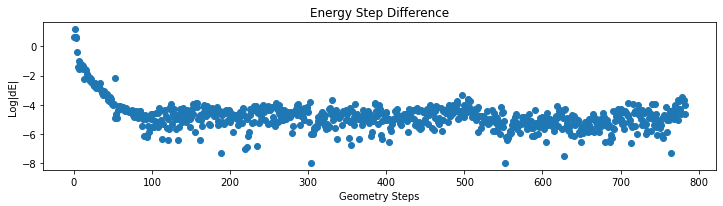
\includegraphics[scale=0.5]{Figures/Analysis/IVDW/D2_Energy_Force_Step1.png}
    \caption{Change in Energy between Step}
    \label{fig:energy_step}
    \vspace{10 mm}
\end{subfigure}
\vspace{10 mm}
\begin{subfigure}{1\textwidth}
    \centering
    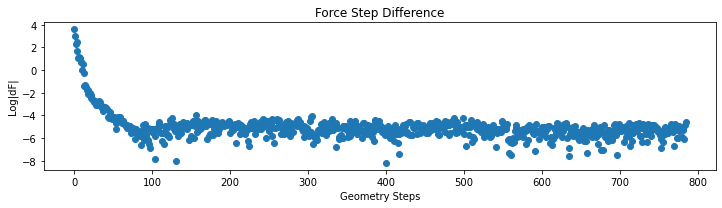
\includegraphics[scale=0.5]{Figures/Analysis/IVDW/D2_Energy_Force_Step2.png}
    \caption{Change in Force between Step}
    \label{fig:force_step}
\end{subfigure}
\captionsetup{font = footnotesize, justification = centering}
\caption[Changes in Energy and Force Between each Optimisation Step]{Changes in Energy and Force between each optimisation step. It is evident that a significant part of the optimisation is spent close to the correct solution but only achieves it after quite some time.}
\label{fig:energy_force_step}
\end{figure}

\subsubsection{Convergence}
\label{subsubsec:convergence}
The number of k\nobreakdash-points along each axis and the plane wave cut\nobreakdash-off energy are two calculation parameters that must be optimised to find sensible values before the main calculation can begin. This occurs through increasing these parameters until no significant change of the energy of the system is detected. \Cref{fig:convergence_params} demonstrates this process for an \acrshort{alm} calculation performed in this work. The Monkhurst\nobreakdash-Pack k\nobreakdash-points grids were 715, 826 and 937 in each reciprocal lattice coordinate respectively. Any increase from the first group resulted in a change in the energy of the system of less than \SI{0.001}{eV} which was deemed not enough to justify the additional computational time. The plane wave cut\nobreakdash-off energy was varied between 600 and \SI{1200}{eV} and was selected to be \SI{900}{eV}, where an increase resulted in a change of less than \SI{0.01}{eV} to the energy of the system. 

\begin{figure}
\begin{subfigure}{1\textwidth}
    \centering
    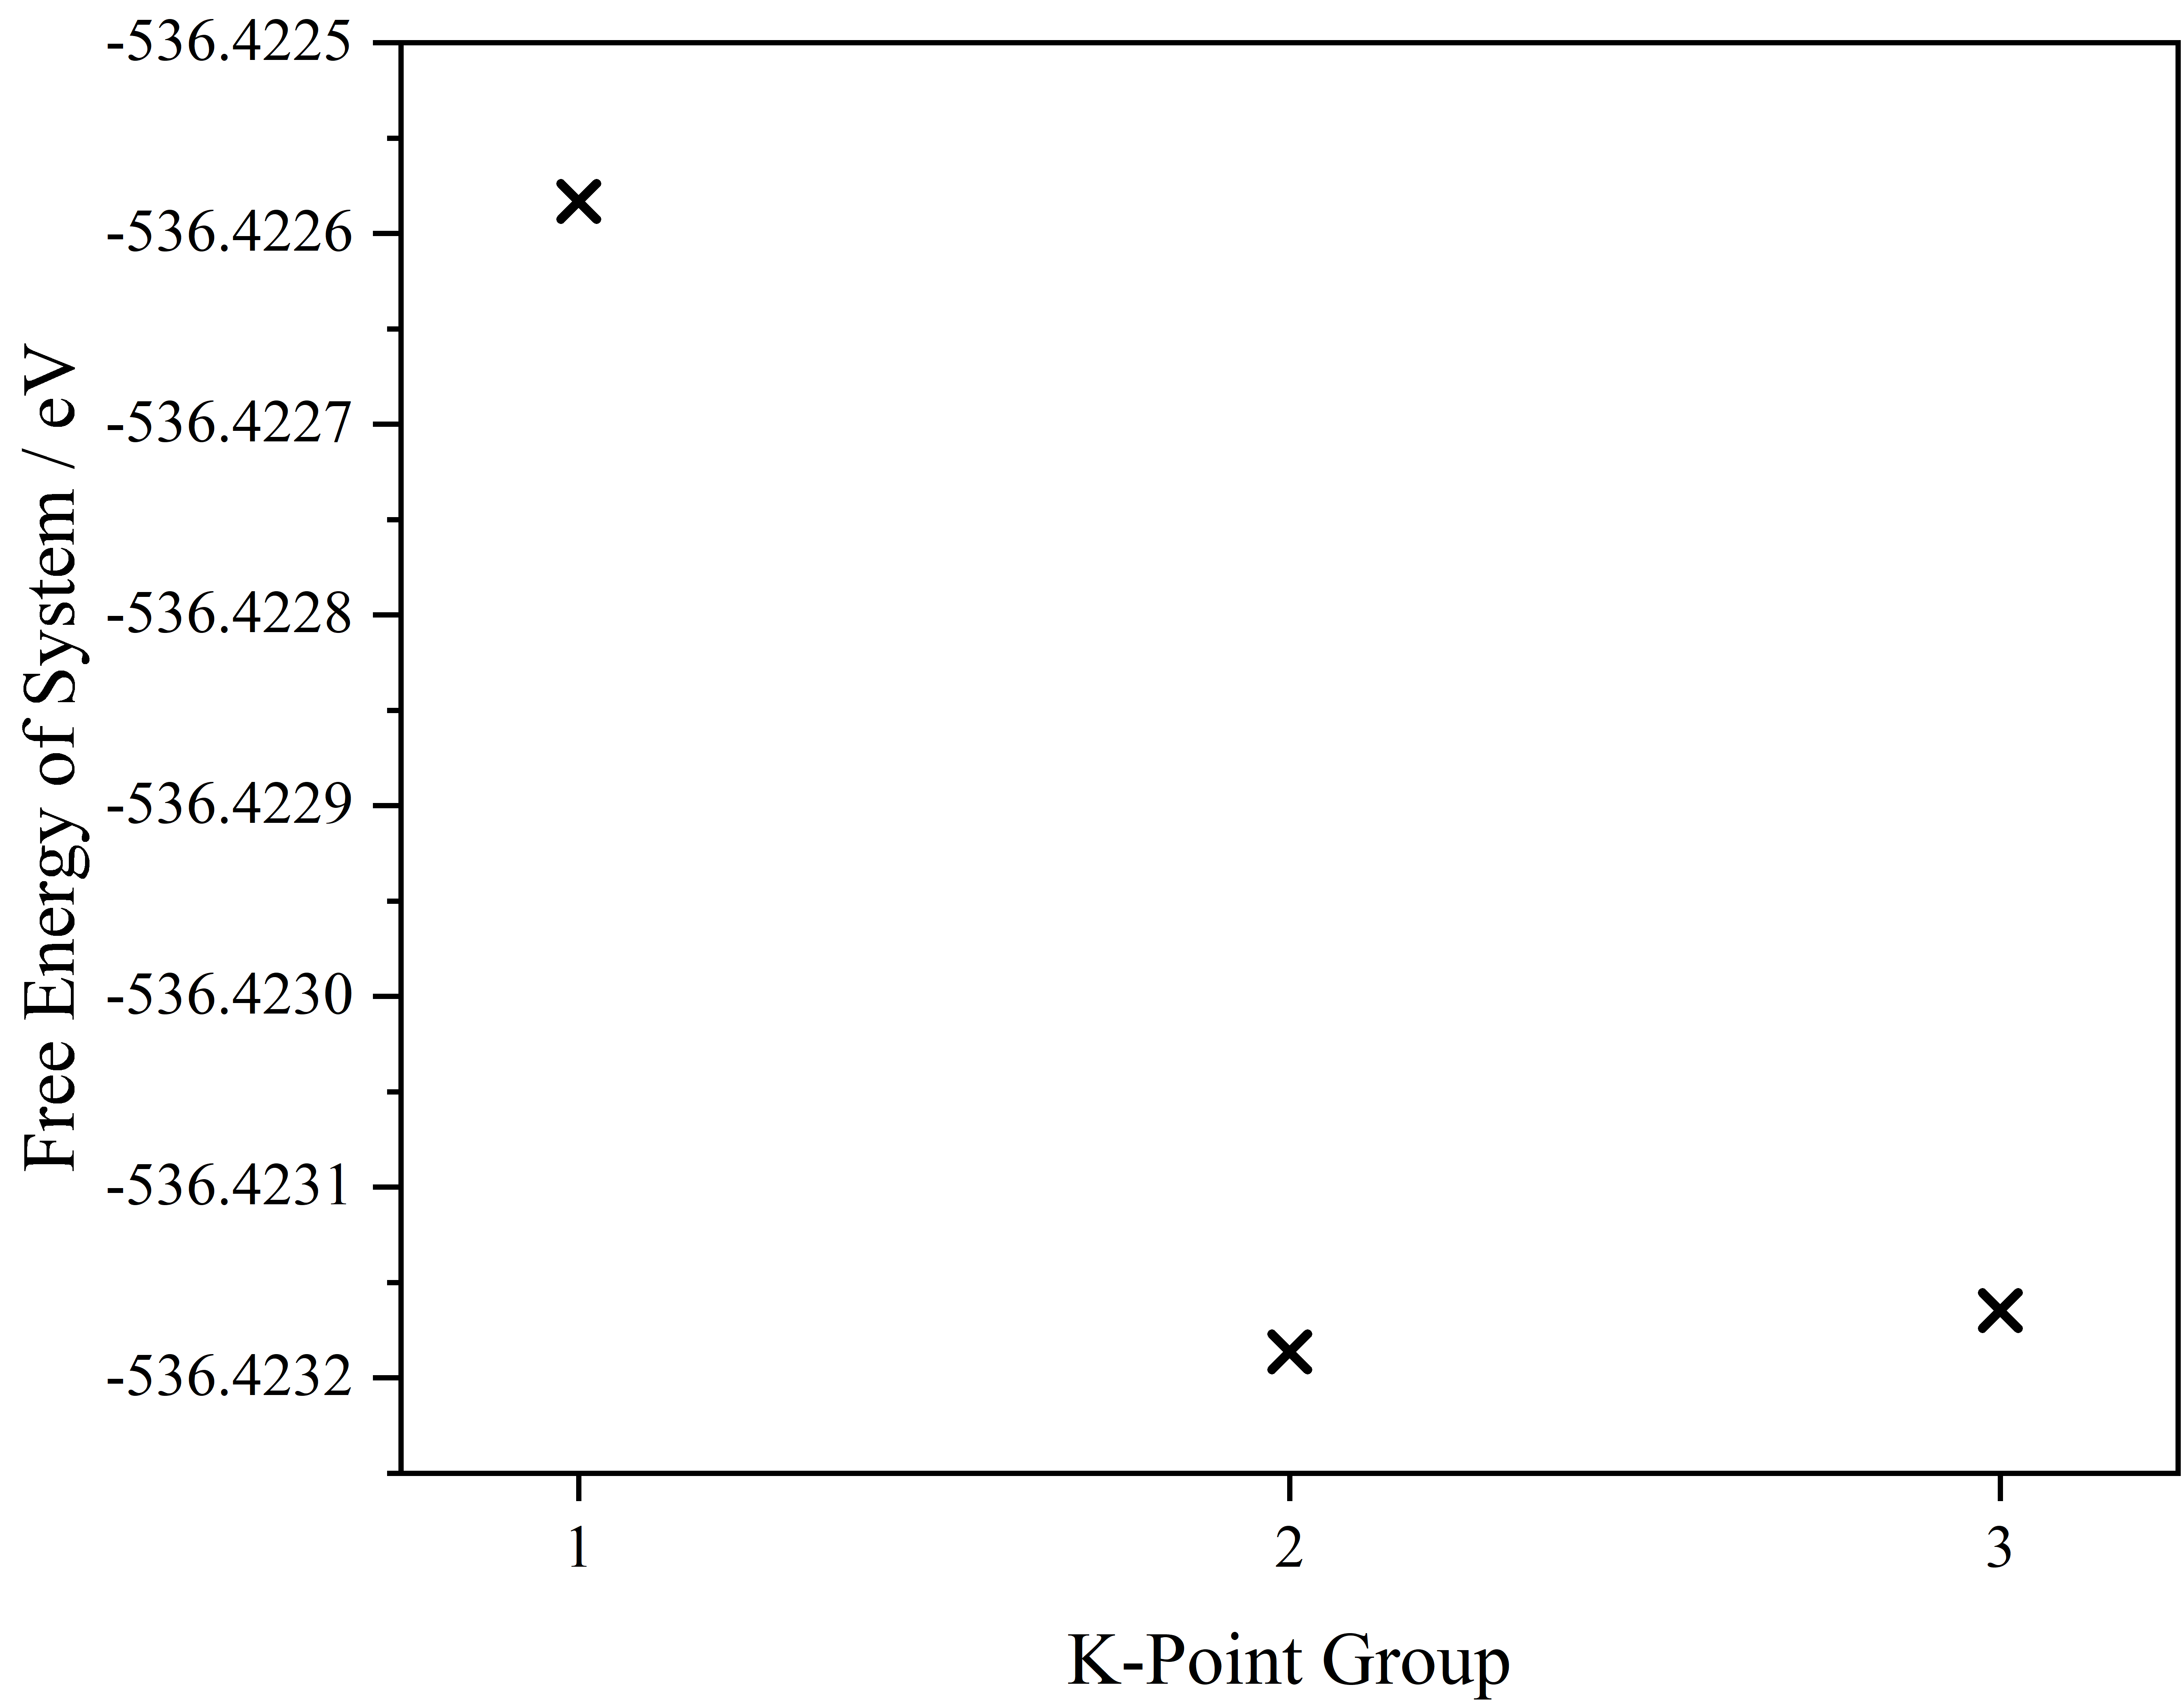
\includegraphics[scale=0.4]{Figures/Misc/IVDW/KPTConG.png}
    \caption{K-Point Convergence}
    \label{fig:kpt_convergence}
    \vspace{10 mm}
\end{subfigure}
\vspace{10 mm}
\begin{subfigure}{1\textwidth}
    \centering
    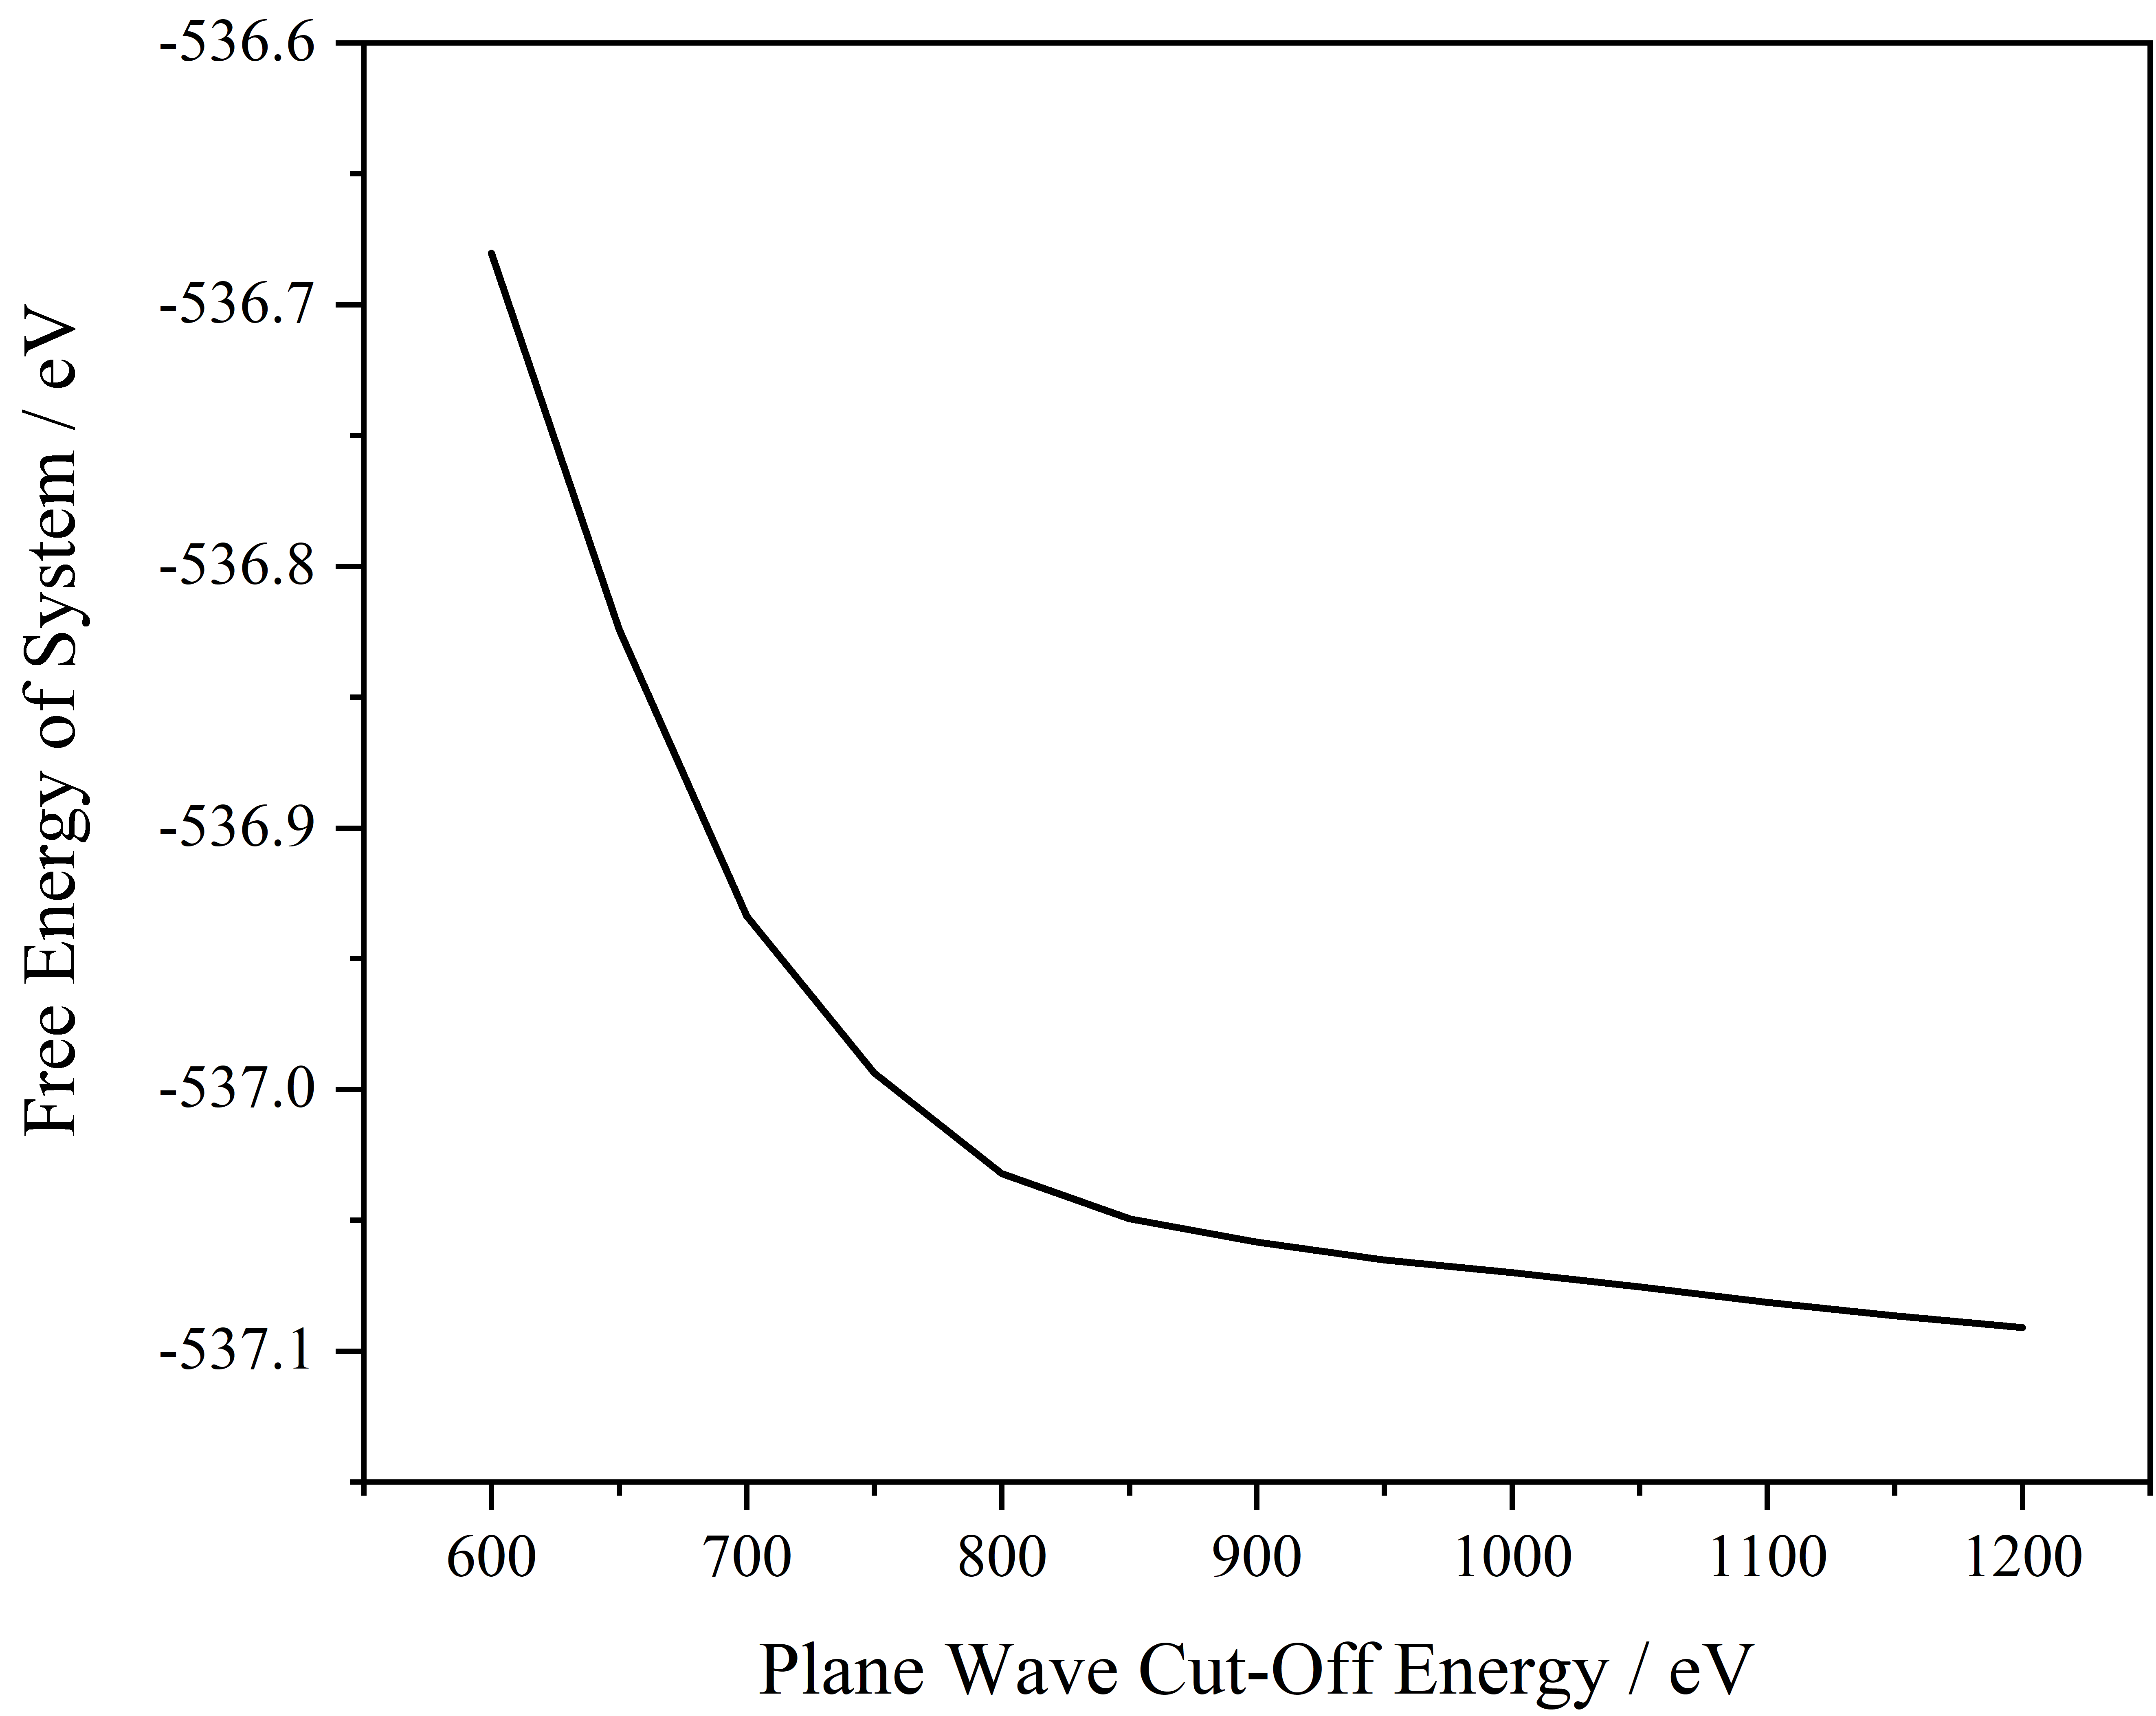
\includegraphics[scale=0.4]{Figures/Misc/IVDW/CutOffEConG.png}
    \caption{Cut-Off Energy Convergence}
    \label{fig:EC_convergence}
\end{subfigure}
\captionsetup{font = footnotesize, justification = centering}
\caption[The Convergence of the Plane Wave Cut-Off Energy and Number of K-points]{The convergence of the plane wave cut\nobreakdash-off energy and number of k\nobreakdash-points for an \acrshort{alm} calculation. The first k\nobreakdash-point group and \SI{900}{eV} were selected for all subsequent calculations on the \acrshort{alm} system.}
\label{fig:convergence_params}
\end{figure}

One method of examining whether suitable parameters have been chosen is to check the first three modes. These will represent translation of the entire unit cell in each Cartesian coordinate and when the system is simulated with complete accuracy then these modes should be as close to zero frequency as possible. This is owing to the identical nature of each unit cell which means when an ion is translated to the same position in a neighbouring unit cell, it should have the same energy. In practice, this is not the case owing to the finite number of k\nobreakdash-points used to sample the \acrshort{bz}. This results in small changes in the energy of the system when considering translation which manifest as non\nobreakdash-zero frequencies. These can be projected out~\cite{Louck1976} and ignored but can serve as a useful measure of how well suited the calculation parameters were. If the k\nobreakdash-point grid is not fine enough, then these translational modes will be large (>~\SI{0.2}{\acrshort{thz}}) and this is an indication that the frequencies for the vibrational modes of interest will be inaccurate. Whilst these will never be exactly zero, small values below this are generally considered acceptable~\cite{Kendrick2020}.

\subsubsection{Starting Structures}
Starting structures are usually obtained from X-ray or neutron diffraction patterns. This means, when obtaining a structure, it is desirable to perform the measurement at as low a temperature as possible. The resulting structure will be closer to its ground state than it otherwise would have been and this reduces the likelihood of finding a local minimum instead of the global one. Neutron diffraction patterns are preferred as the accuracy of the positions of H atoms will be much higher and so the optimisation will often be quicker and more accurate. However, these are much less common and so \acrfull{xrd} patterns tend to be used. 

\subsubsection{Packages}
There are many \acrshort{dft} calculation and post-processing packages that can be used for this purpose~\cite{Clark2005, Gale2011, dovesi2020crystal} but this work will use the VASP~\cite{Hafner2008} \acrshort{dft} package to optimise all atomic positions and unit cell dimensions for all calculations in this work. The dynamical matrix and Born effective charges were also calculated using Phonopy~\cite{Togo2015} which uses VASP as its computational engine. This group has used many packages including CASTEP~\cite{Clark2005}, VASP and Crystal17 to calculate \acrshort{thz} absorption spectra with success using all three packages. VASP was chosen here as the inclusion of its \acrshort{paw} pseudopotentials mean that a lower plane wave cut\nobreakdash-off energy is required than the equivalent CASTEP calculation. Previous calculations have also shown VASP tends to be less sensitive to k\nobreakdash-point grid size than some of the other codes. As such this, coupled with the ability of Phonopy to use VASP and improve the efficiency of phonon calculations makes VASP an ideal choice for calculations of these large systems.

\subsection{Construction of the Simulated Spectrum}
\label{subsec:pdielec}
PDielec~\cite{Kendrick2016}, is a DFT and molecular mechanics post\nobreakdash-processing package for solid\nobreakdash-state applications that enables calculation of IR and THz spectra of a material. This reads in phonon frequencies and normal modes from a wide range of codes while calculating the the mode intensities using the Born effective charges calculated for the given system. In turn the methods included also enable experimental effects such as scattering, particle size, shape and orientation along with experimental sampling method to try and improve the correlation between calculation and experiment. These methods are described in more detail by Kendrick and Burnett~\cite{Kendrick2016, Kendrick2020, john_kendrick_2022_5888313} but will be summarised here. The Born effective charge tensor is used to calculate the oscillator strength tensor~\cite{Gonze1997}. The trace of this tensor, which is the sum across the diagonal, for a given transition is equal to the intensity of that transition.
Whilst each mode is associated with a frequency and an intensity, this is not directly comparable with experiment. In vibrational spectroscopy, modes must always have a width and this width causes the absorption mode to have an inherent shape. This shape depends on the properties of the system, such as temperature. At low temperatures, peaks typically demonstrate a Lorentzian peak shape whereas as temperature increases, peak broadening of a Gaussian nature dominates. The transition intensity of the \(j^{th}\) mode, \(I_j\), is related to its integrated molar absorption coefficient, \(A_j\) by~\cite{Wilson1955}:

\begin{equation}
A_j = \frac{N \pi}{3 c^2 log_e 10} g_j I_j
\end{equation}

where \(N\) is the number of molecules per unit volume, \(c\) is the speed of light and \(g_j\) is the degeneracy of the mode. This, assuming a Lorentzian shape, can be related to the peak's \acrfull{fwhm}, \(\sigma_j\) by:

\begin{equation}
a_j(\bar{\nu}) = \frac{2 A_j}{\pi} \frac{\sigma_j}{4(\bar{\nu} - \bar{\nu}_j)^2 + \sigma_j^2}
\end{equation}

These peak widths are set within PDielec and can be set to all have the same value or can be individually optimised.

Owing to the powdered nature and potential dilution of the sample used to produce the experimental spectrum that the calculation is attempting to reproduce, these properties must be incorporated otherwise the intensities of the modes will be inaccurate. The dilution can be accounted for using an effective medium approximation and is shown for ZnO in \Cref{fig:ConcPDGUI}. These figures have been generated using calculations of ZnO provided as a simple example within the latest PDielec release~\cite{john_kendrick_2022_5888313}.

\begin{figure}
    \centering
    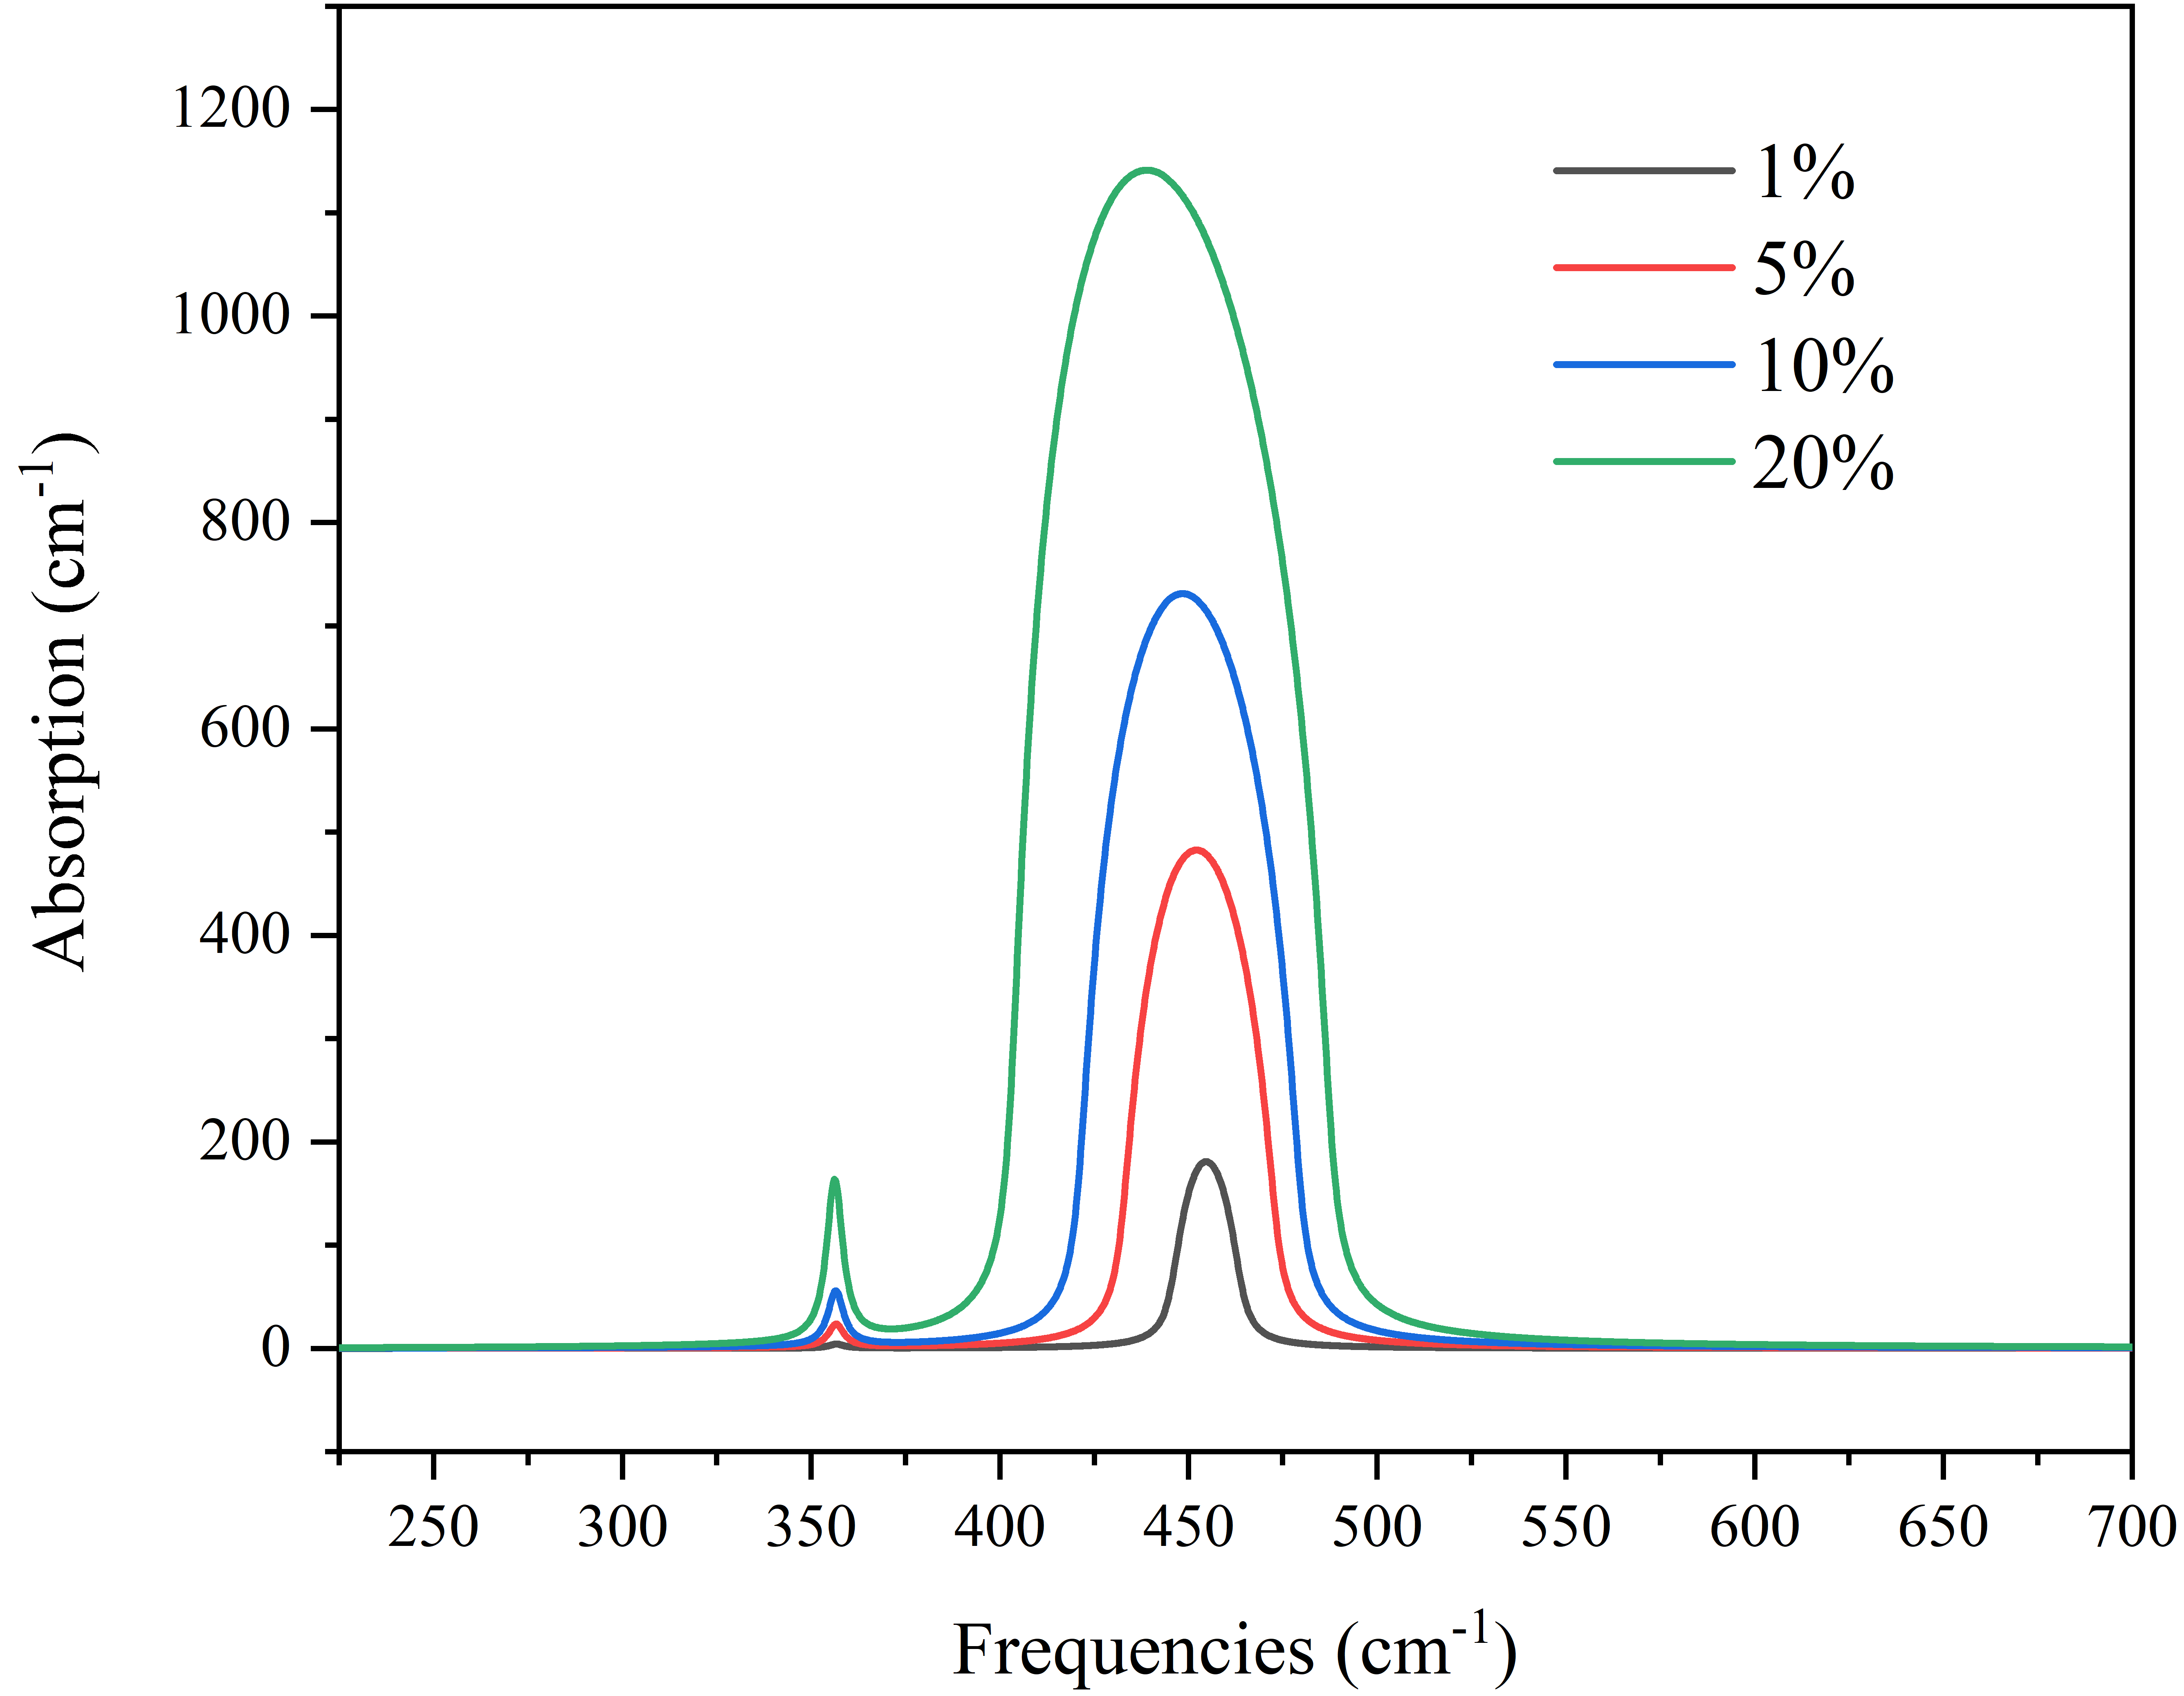
\includegraphics[scale=0.6]{Figures/Misc/Theory/ConcentrationG.png}
    \captionsetup{font = footnotesize, justification = centering}
    \caption[The Effect of Concentration on the Calculated THz Absorption Spectrum of ZnO]{The effect of concentration on the calculated \acrshort{thz} absorption spectrum of ZnO. The peak widths have been set to be constant so any increase is a result of the mixing model.}
    \label{fig:ConcPDGUI}
\end{figure}

The effect of not being a single crystal and the dilution medium on the absorption is also modelled through the use of effective medium theories such as the Maxwell\nobreakdash-Garnett or Bruggerman mixing rules which allow the composite material to be treated as a homogeneous mixture. The effect of particle shape and choice of theory is depicted in \Cref{fig:EMAsShapes} where a range of combinations of crystallite shapes and effective medium theories are shown. A more detailed comparison between these theories was done by Kendrick and Burnett~\cite{Kendrick2020} but this arises from the interaction between the phonons and the incident radiation where charges form on the surface of the crystallites which affect the oscillation frequency of these phonons. 

\begin{figure}
    \centering
    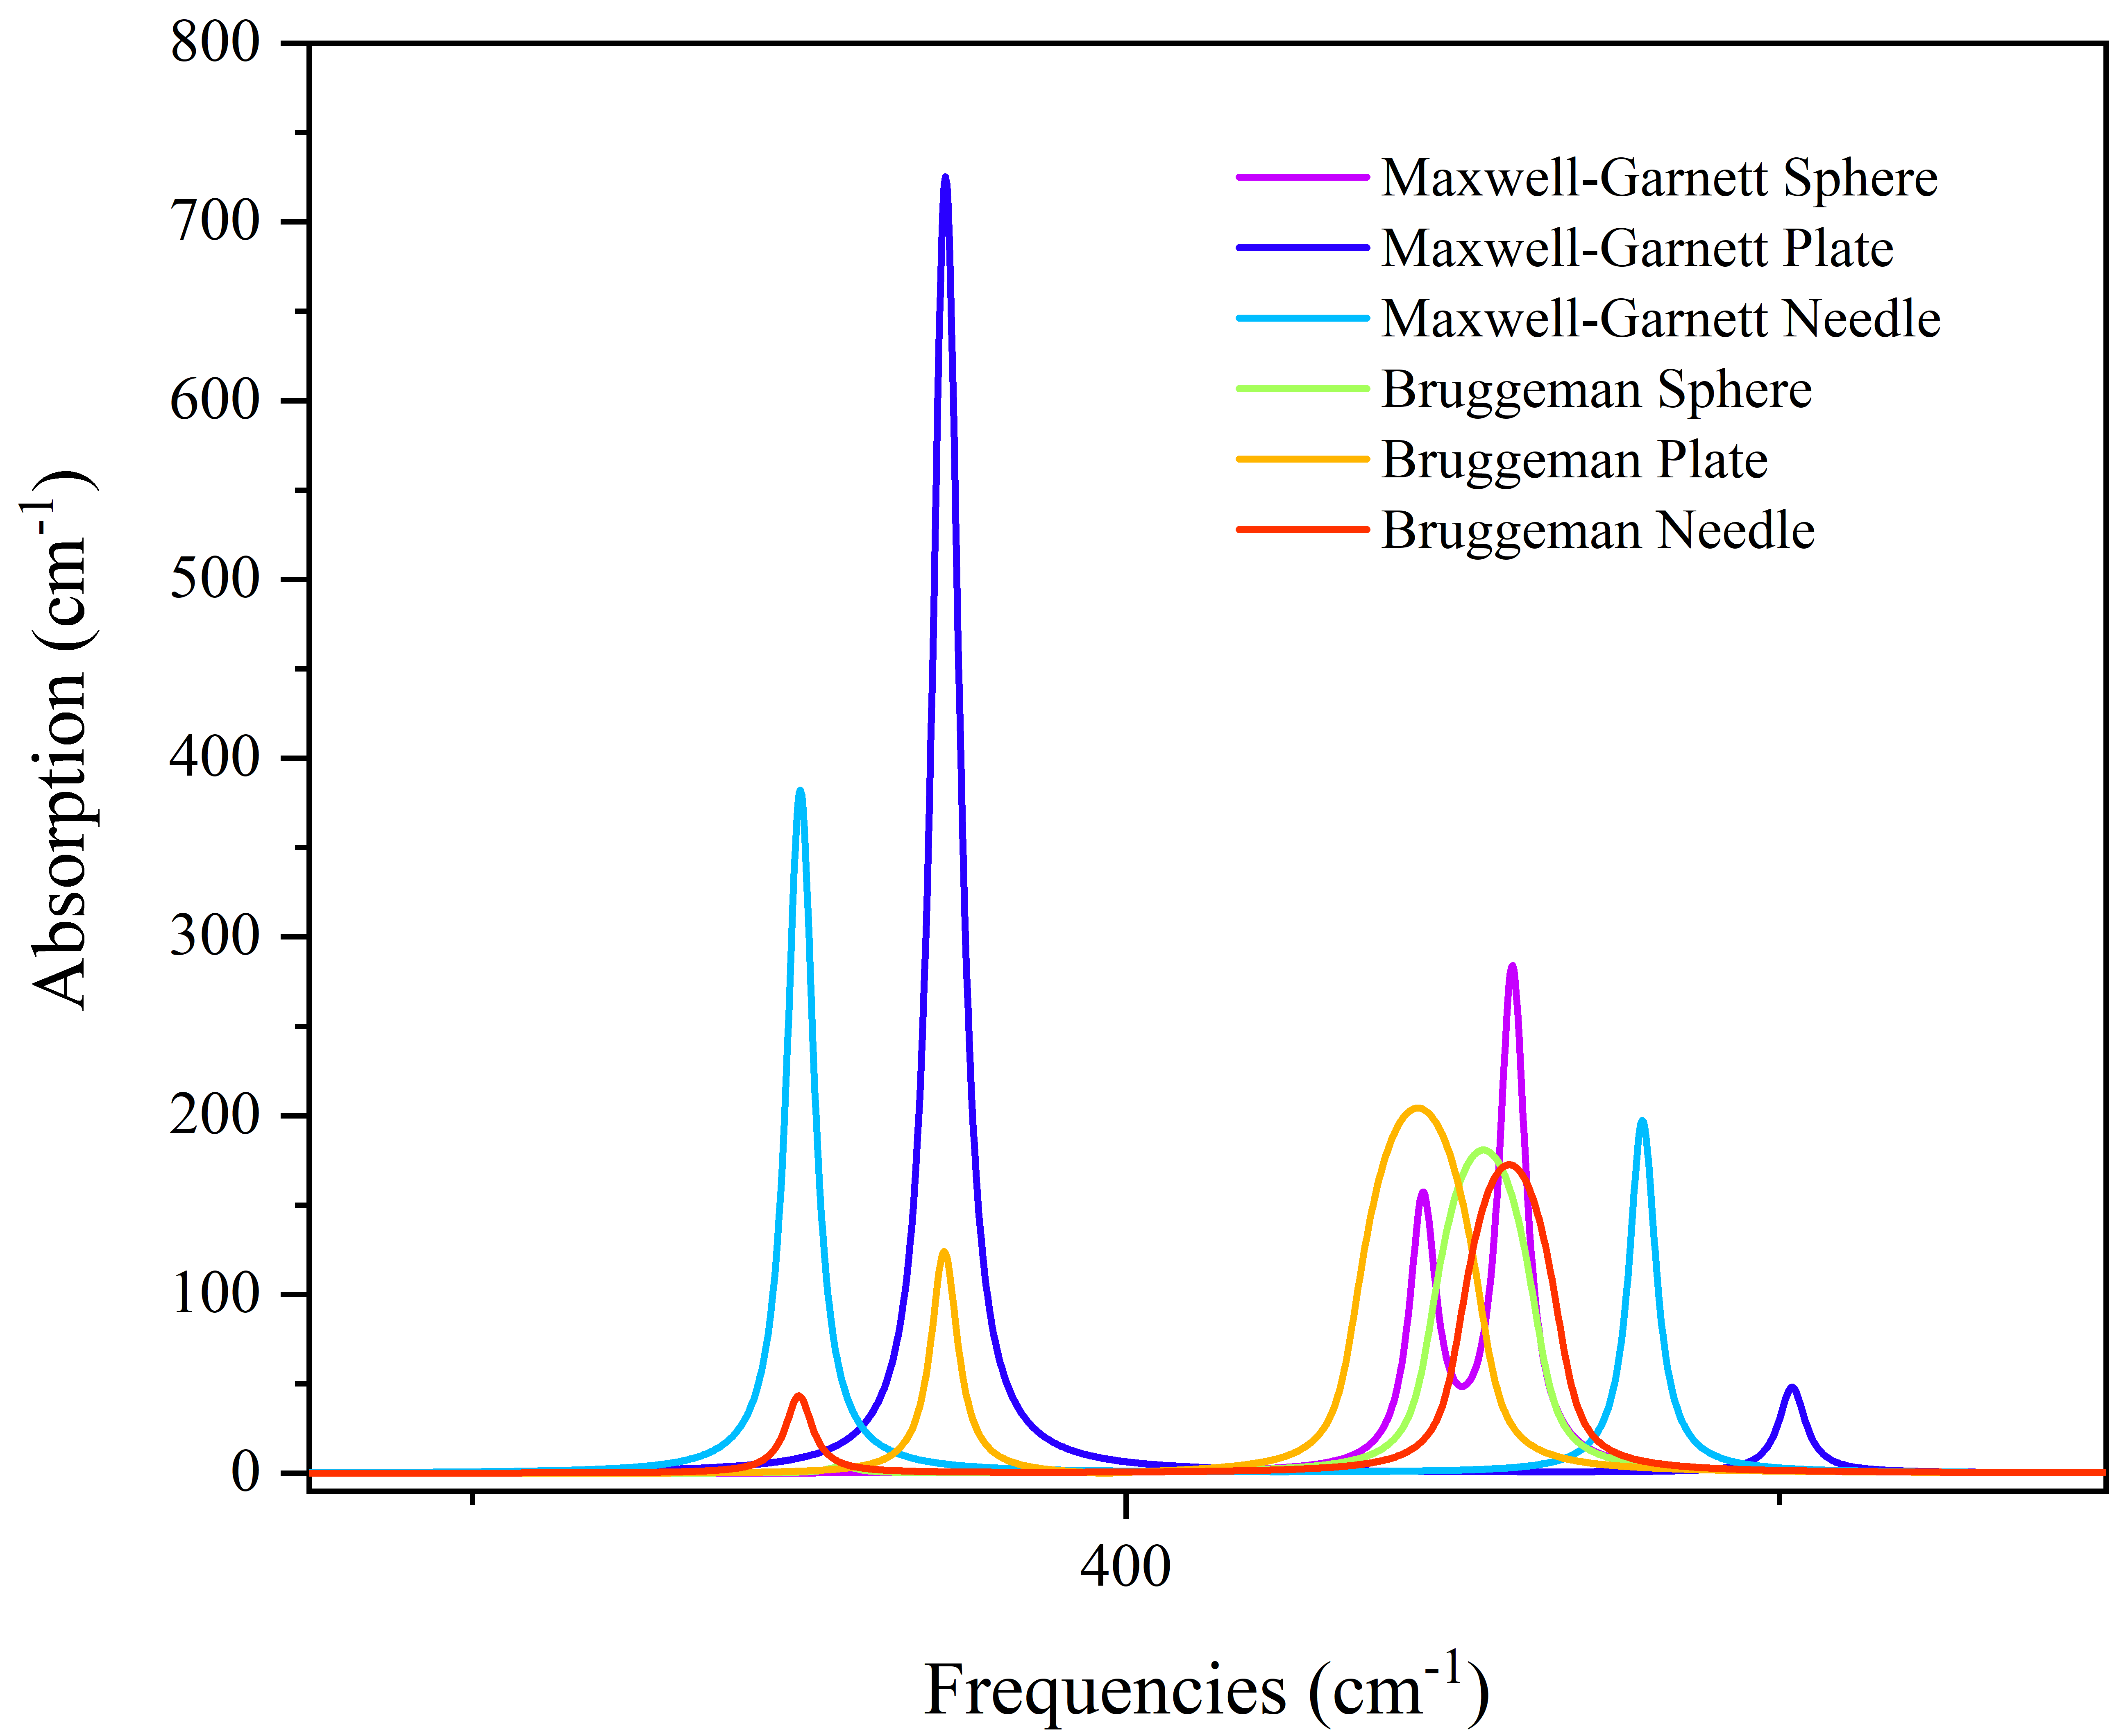
\includegraphics[scale=0.6]{Figures/Misc/Theory/ZnOMRG.png}
    \captionsetup{font = footnotesize, justification = centering}
    \caption[A Comparison between Crystallites of Different Shapes using the Bruggerman and Maxwell-Garnett Effective Medium Approximations]{A comparison between the calculated \acrshort{thz} absorption spectra of crystallites with different shapes using the Bruggerman and Maxwell-Garnett effective medium approximations.}
    \label{fig:EMAsShapes}
\end{figure}

The effect of air trapped in the medium is significant and must be incorporated to accurately represent the experimental spectrum. This is shown in \Cref{fig:AirEffect}, and two factors must be considered. The air void volume fraction and the air void radius. \Cref{fig:AirEffect} shows that the radius dominates the background absorption, especially in the region below \SI{300}{cm^{-1}} which is currently accessible using our \acrshort{tds} systems. PDielec is including Mie scattering to take into account the scattering of light by the air voids and this is what mostly contributes to the rising background absorption seen in the majority of the \acrshort{thz} absorption spectra in this thesis. Further discussion of the importance of including some of these parameters when post\nobreakdash-processing with PDielec will take place in \Cref{ch:ivdw}.

\begin{figure}
    \centering
    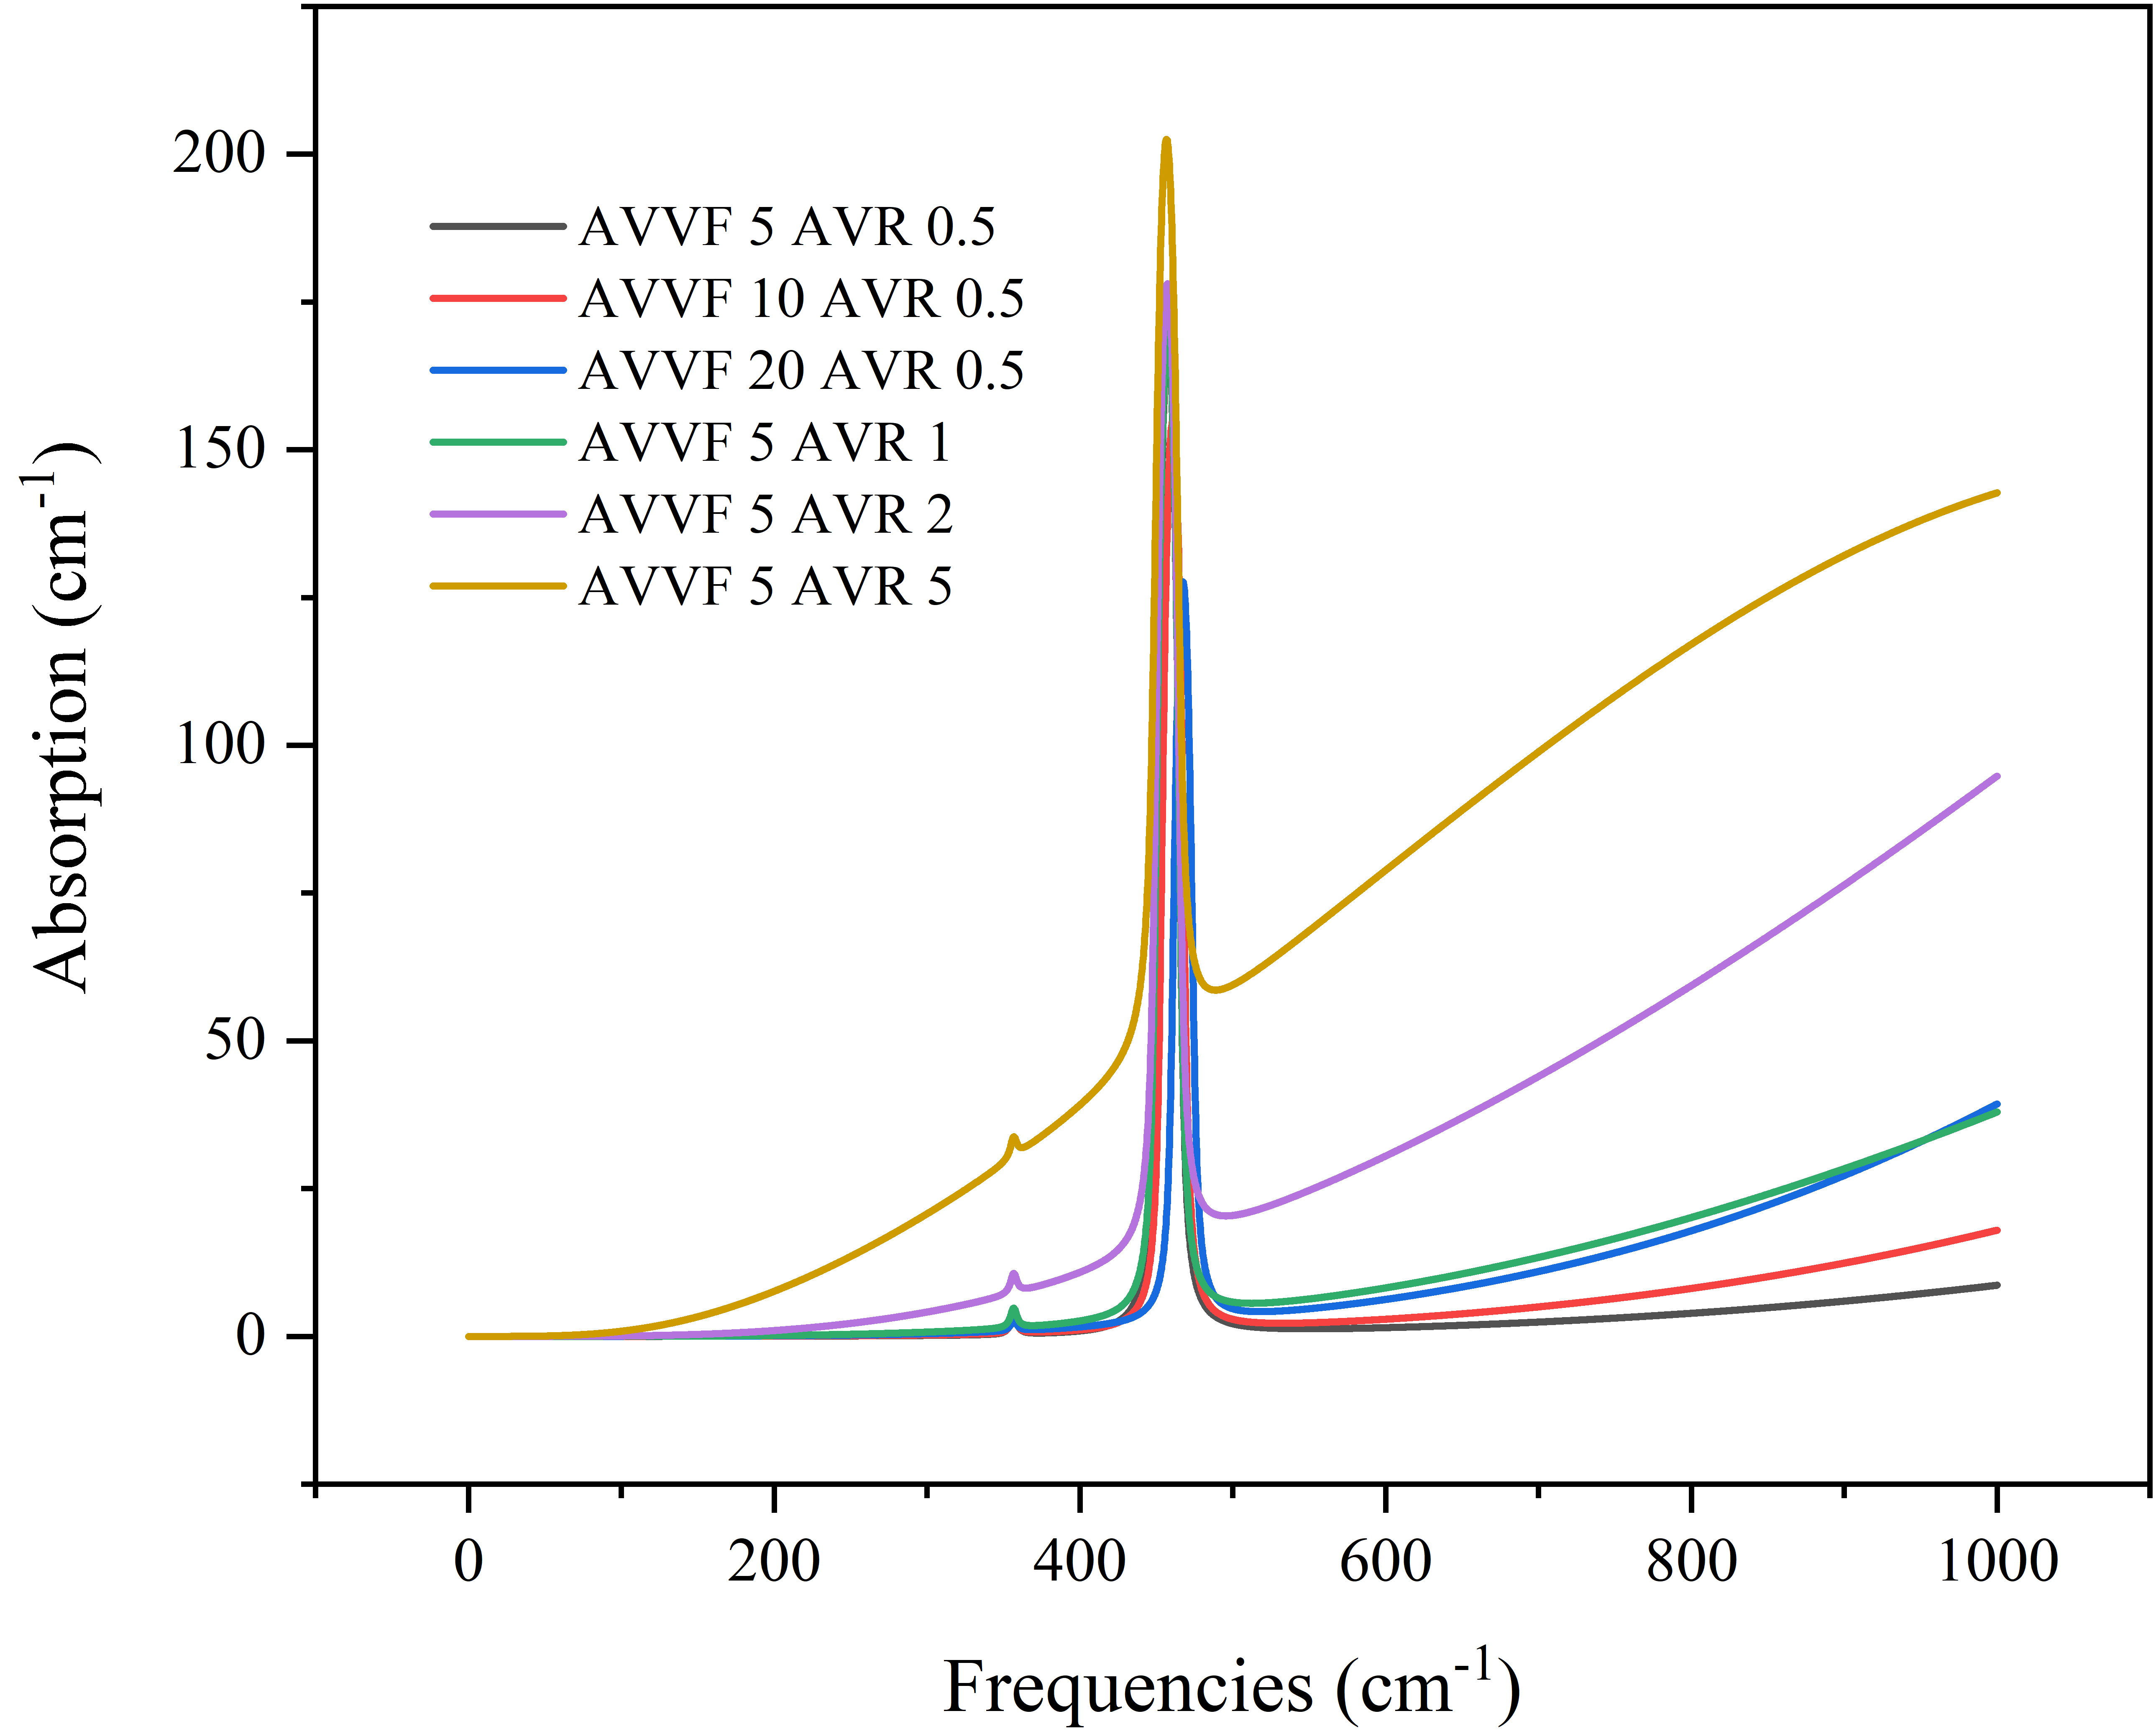
\includegraphics[scale=0.6]{Figures/Misc/Theory/EffectOfAirG.png}
    \captionsetup{font = footnotesize, justification = centering}
    \caption[The Effect of Air void Volume Fraction and Air Void Radius on a Calculated THz Absorption Spectrum]{The effect of air void volume fraction and air void radius on a \acrshort{thz} absorption spectrum.}
    \label{fig:AirEffect}
\end{figure}

\subsection{Generalised Calculation Workflow}
\Cref{fig:workflow} shows a detailed flowchart of the calculation process. The area in blue shows how the files were set up to begin testing for convergence. The area in green describes the convergence testing process and how parameters were iteratively increased until they were satisfactory. Finally, the area in red describes the process of optimising the unit cell and ionic positions and subsequent calculation of the dynamical matrix and Born effective charges. This is a generalised flowchart that includes a check as to whether these latter parameters could finish within 48 hours whilst using \acrshort{dfpt} in VASP. If not, then Phonopy was used instead. The output was then processed in PDielec.

\begin{figure}
    \centering
    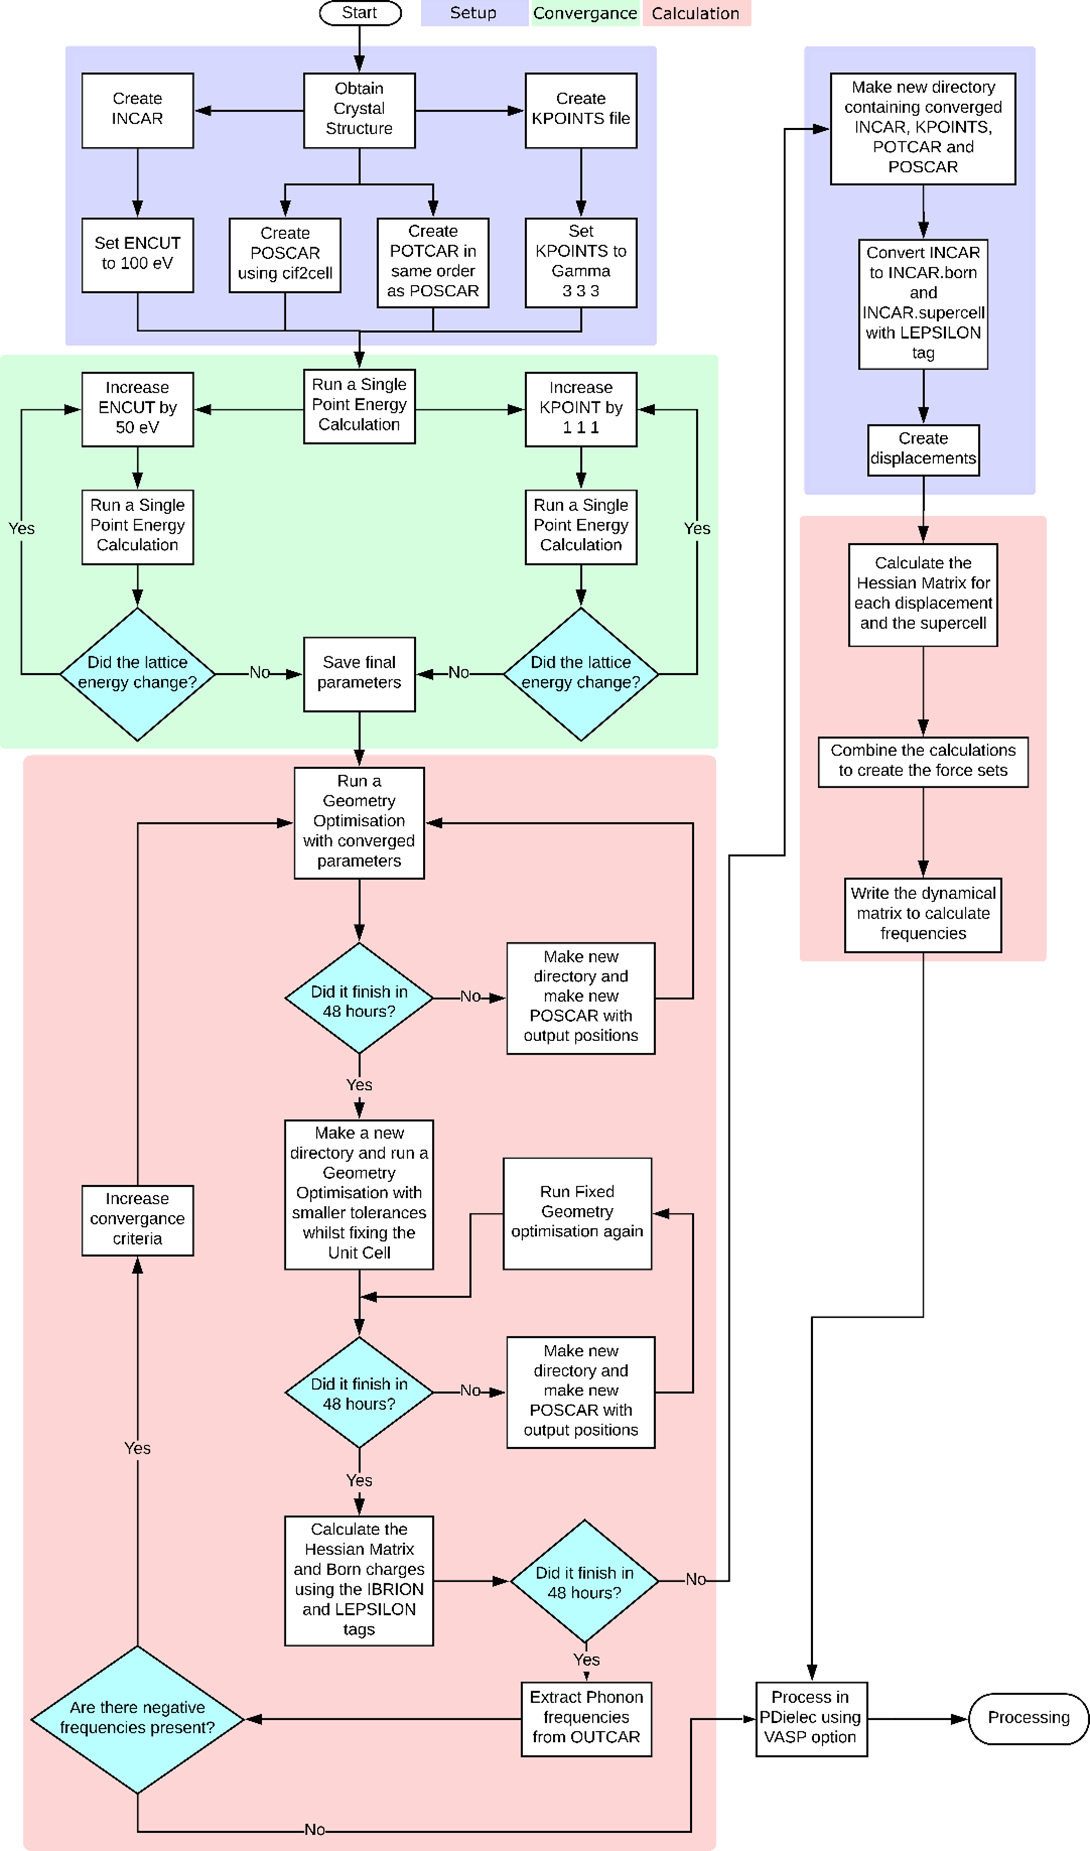
\includegraphics[scale=1.08]{Figures/Misc/Theory/VASP_Phonopy Workglow.png}
    \captionsetup{font = footnotesize, justification = centering}
    \caption[A Flowchart Depicting the Calculation Process]{A flowchart depicting the set-up of files, convergence testing and main calculation process of a \acrshort{dft} calculation.}
    \label{fig:workflow}
\end{figure}

\section{Conclusion}
This chapter described \acrshort{dft} and the principles and challenges behind its implementation. The process of creating a comparable theoretical spectrum was also detailed. \acrshort{dft} calculations are used extensively in \Cref{ch:ivdw} and \Cref{ch:qha} and will be discussed further there.